\documentclass[../CSC_5RO06_TA.tex]{subfiles}

\begin{document}
\section*{Question 3}

Vivaldo HLS est un outil qui facilite la mise en œuvre de circuits personnalisés sur FPGA, permettant aux développeurs de travailler avec un niveau d'abstraction plus élevé des composants du système. Ce logiciel prend en compte les caractéristiques du circuit FPGA souhaité pour effectuer une simulation des propriétés en exécution réelle, en estimant ses performances et son utilisation des ressources. En simulant son comportement, il est possible de générer un résumé des attributs, présentant des données telles que les temps de latence, les performances et les ressources matérielles utilisées. Le procédé permet aux développeurs de mieux comprendre les caractéristiques d'implémentation d'un algorithme dans un circuit, sans l'implémenter de facto en physique, ce qui représente un gain de temps et évite l'écrasement répétitif des configurations de circuit.

Dans le cadre de l'estimation des paramètres du circuit FPGA trouvé sur le Zedboard, pour les algorithmes C++ les plus performants considérés dans la section précédente, la synthèse de chacun a été générée pour différentes tailles de puces.

Pour cela, certaines des optimisations disponibles pour ce type de systèmes ont été utilisées, afin de comparer l'effet que chacune d'elles a sur les algorithmes décrits ci-dessus.

Avant de présenter les résultats de chacun des algorithmes, un bref résumé de chacun des algorithmes utilisés pour cette étude est présenté :

\textbf{Aucune optimisation :}  C'est le code de base qui effectue la multiplication matricielle qui
 N'inclut pas les optimisations. Il lit simplement les matrices d'entrée du flux, les multiplie à l'aide de l'algorithme défini et écrit les résultats dans le flux de sortie.

\textbf{Pipeline :}  La directive \textit{\# pragma HLS PIPELINE} est introduite dans plusieurs parties du code, notamment dans les boucles de lecture et de multiplication de la matrice. Cette politique permet aux itérations de boucle de se chevaucher, ce qui améliore la latence en permettant au matériel d'effectuer des opérations en parallèle plutôt que séquentiellement. Le pipeline permet une meilleure utilisation des ressources et une accélération du temps d'exécution, puisque les opérations de lecture, de multiplication et d'écriture peuvent se produire simultanément.

\textbf{Pipeline avec partitionnement de tableau :}  En plus du canalisation dans les boucles, la directive \textit{\# pragma HLS ARRAY\_PARTITION} est utilisée pour diviser complètement les tableaux A et B. Le partitionnement des tableaux signifie que les éléments des tableaux sont accessibles en parallèle, ce qui réduit considérablement la surcharge d'accès à la mémoire. Pour cela, il a été défini que A est complètement partitionné dans la deuxième dimension et B dans la première dimension, ce qui améliore la concurrence dans la multiplication matricielle et augmente les performances.

\textbf{ Pipeline détaillé :}  Dans cette version, la directive \textit{\# pragma HLS PIPELINE activate\_flush rewind} est utilisée dans les boucles. Cela permet des capacités de vidage et de rembobinage, ce qui est utile pour améliorer l'efficacité des boucles itératives, en particulier sur le matériel avec des modèles d'accès cycliques. Cela permet au matériel de mieux gérer le flux continu de données lors des opérations de lecture, de multiplication et d'écriture, minimisant ainsi les temps d'arrêt et améliorant encore la latence du système.


Pour chacune des optimisations, les valeurs des différentes ressources matérielles utilisées dans le FPGA ont été étudiées, en plus du temps d'exécution obtenu avec chacune des combinaisons possibles. Ces ressources sont :

\begin{itemize}
    \item \%BRAM\_18K : Pourcentage de blocs de mémoire BRAM de 18 Kbits utilisés dans le FPGA.
    
    \item \% CSP48E : Pourcentage de blocs DSP utilisés dans le FPGA. Il est notamment spécialisé pour les opérations mathématiques intensives telles que la multiplication et l'addition.
    
    \item \% FF (Flip-Flops) : Pourcentage de bascules (FF) utilisées dans le FPGA.
    
    \item \% LUT (Look-Up Table) : Pourcentage de LUT (Look-Up Tables) utilisées dans le FPGA. Les LUT vous permettent d'effectuer des opérations logiques telles que AND, OR, XOR, etc.
\end{itemize}

Les résultats obtenus pour chaque algorithme sont présentés séparément ci-dessous, avec chacune des optimisations et tailles de matrice qui varient entre 8x8 et 128x128. La raison pour laquelle la taille de la matrice calculée a été réduite est due à la disponibilité de la mémoire et du temps d'exécution disponible.


\subsection{Algorithme Naïve}

\begin{figure}[H]
    \centering
    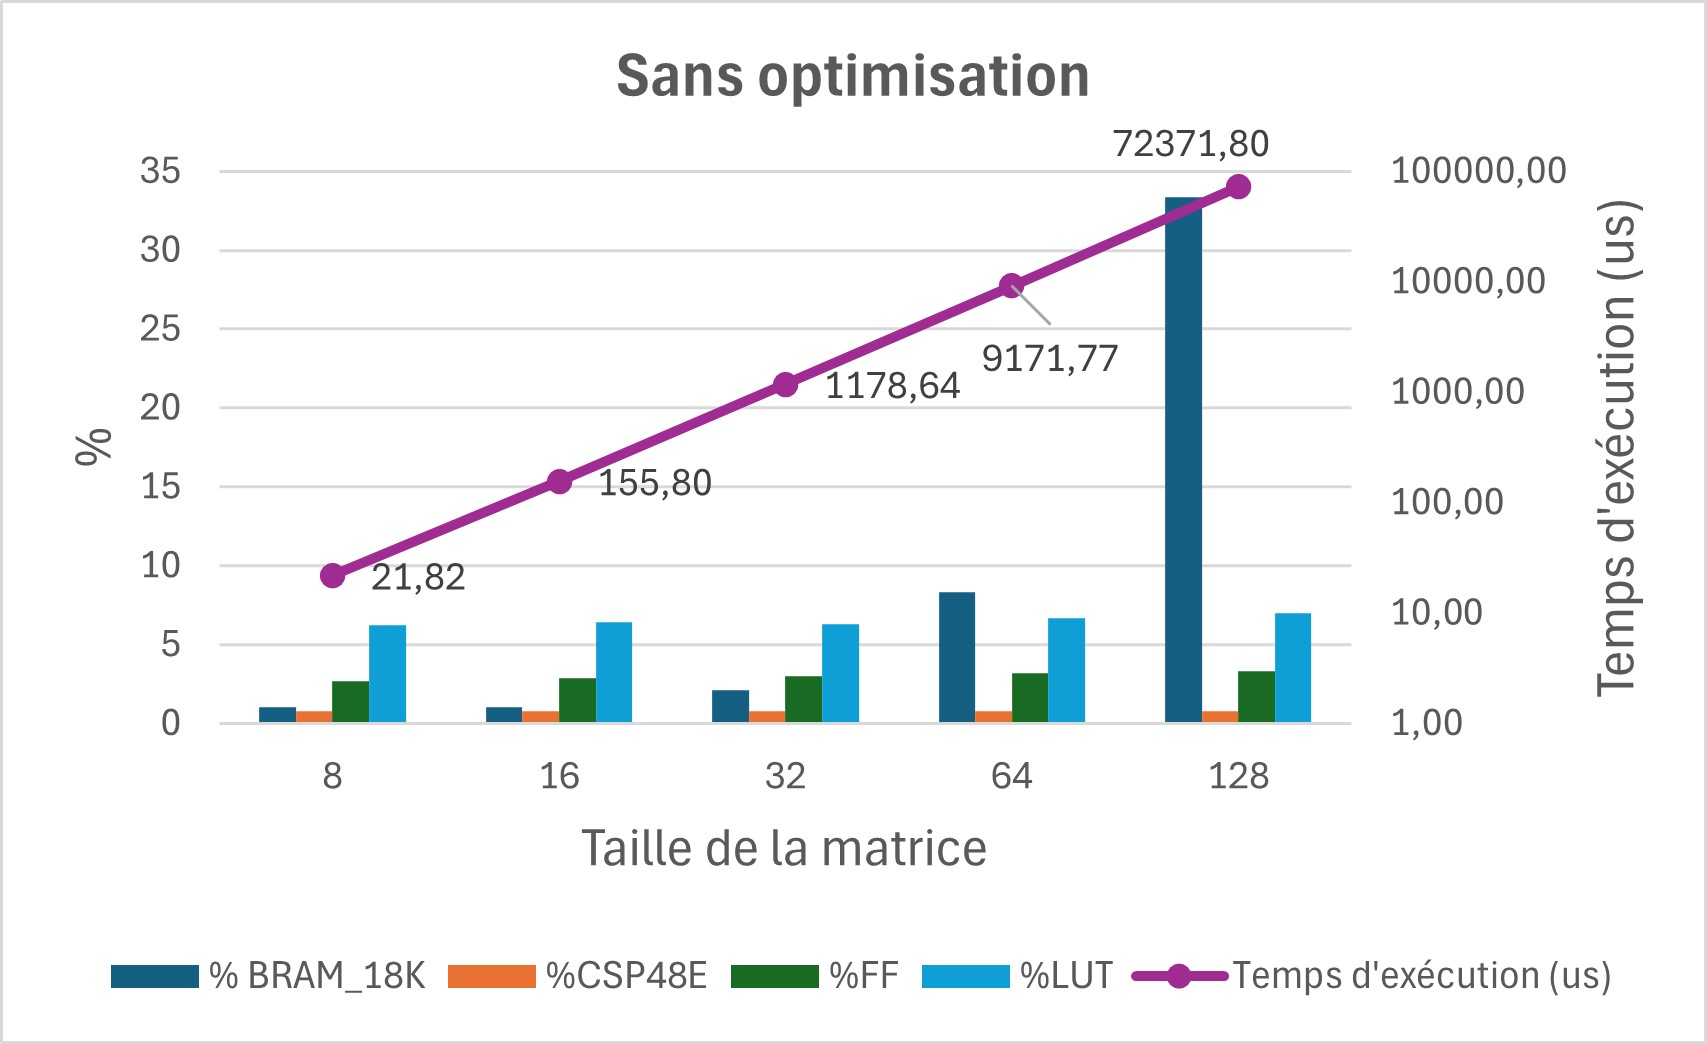
\includegraphics[width=1\columnwidth]{Images/Naive_0.jpg}
    \caption{Naïve sans optimisation.}
    \label{fig:1}
\end{figure}

L'utilisation des ressources (BRAM, CSP48E, FF, LUT) est assez faible, mais le temps d'exécution augmente de façon exponentielle avec la taille de la puce. Cela montre l’inefficacité d’une multiplication naïve sans optimisations, notamment pour de gros volumes de données.


\begin{figure}[H]
    \centering
    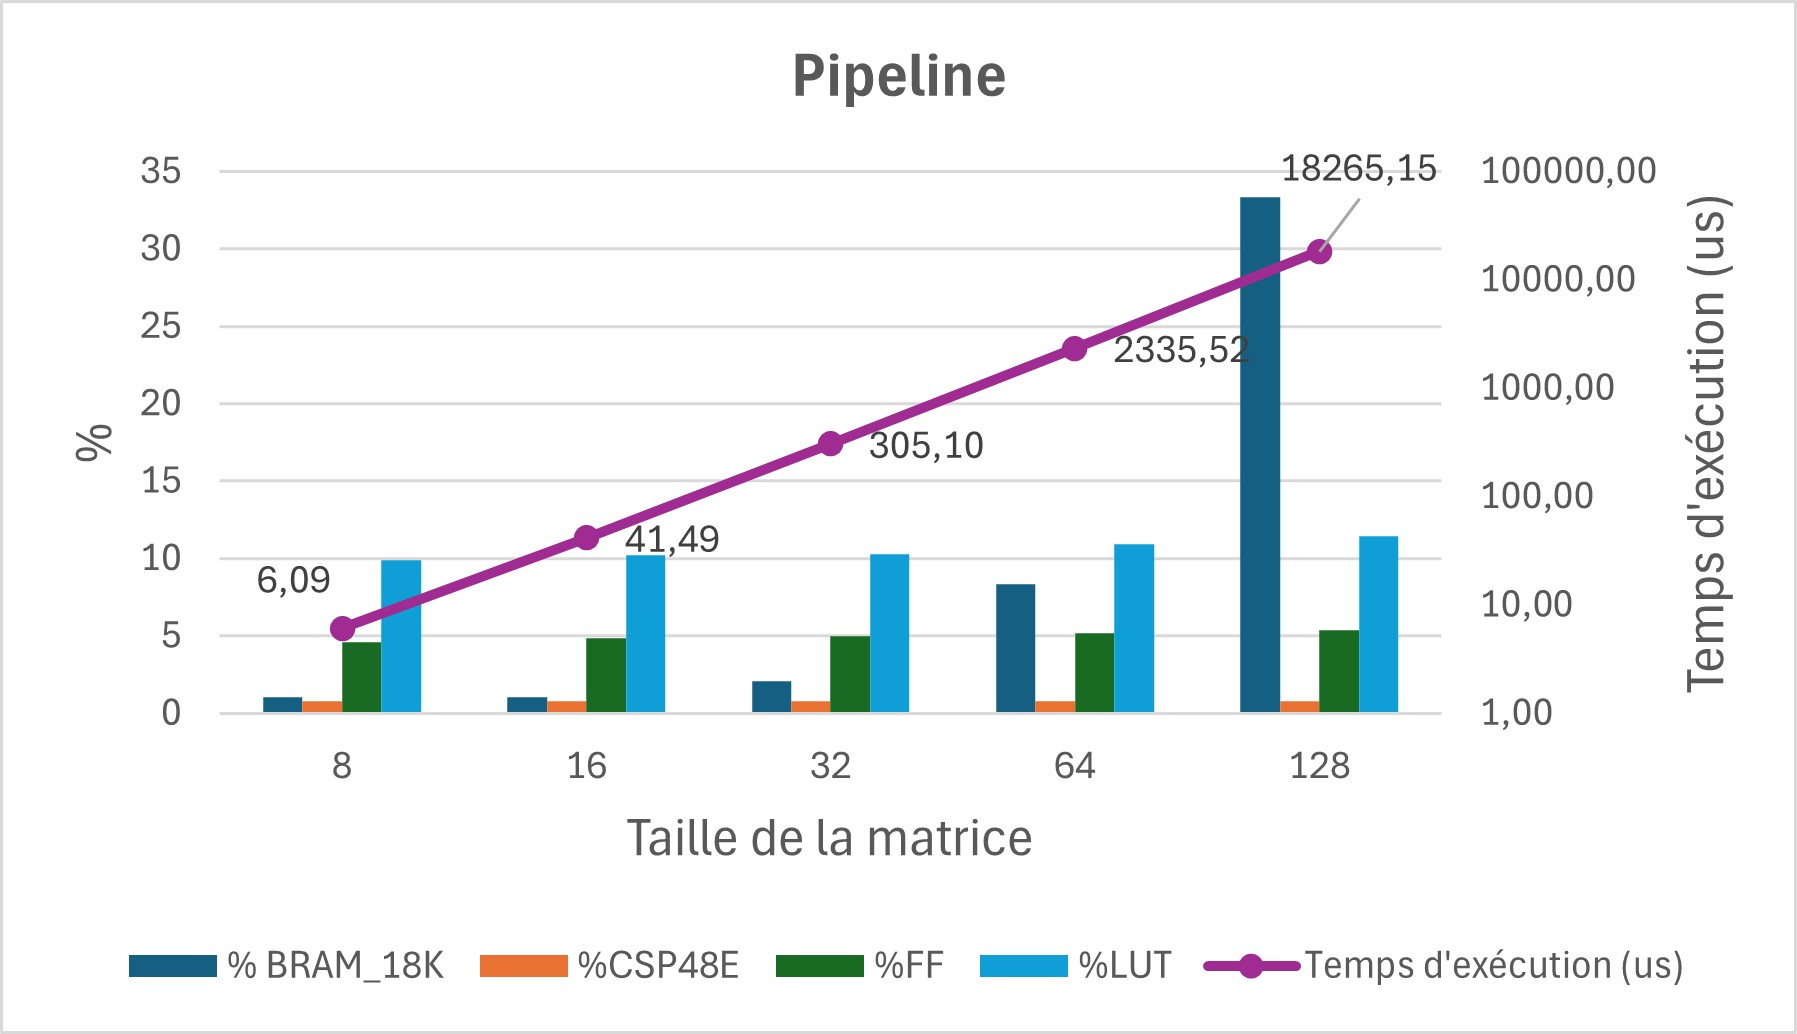
\includegraphics[width=1\columnwidth]{Images/Naive_1.jpg}
    \caption{Naïve avec pipeline.}
    \label{fig:2}
\end{figure}

Le temps d'exécution diminue considérablement. Cependant, le coût est dû à une plus grande utilisation des LUT et des bascules, ce qui indique que le matériel est mieux utilisé pour réduire la latence. Cette optimisation montre un bon équilibre entre l'utilisation des ressources et l'amélioration du temps d'exécution.

\begin{figure}[H]
    \centering
    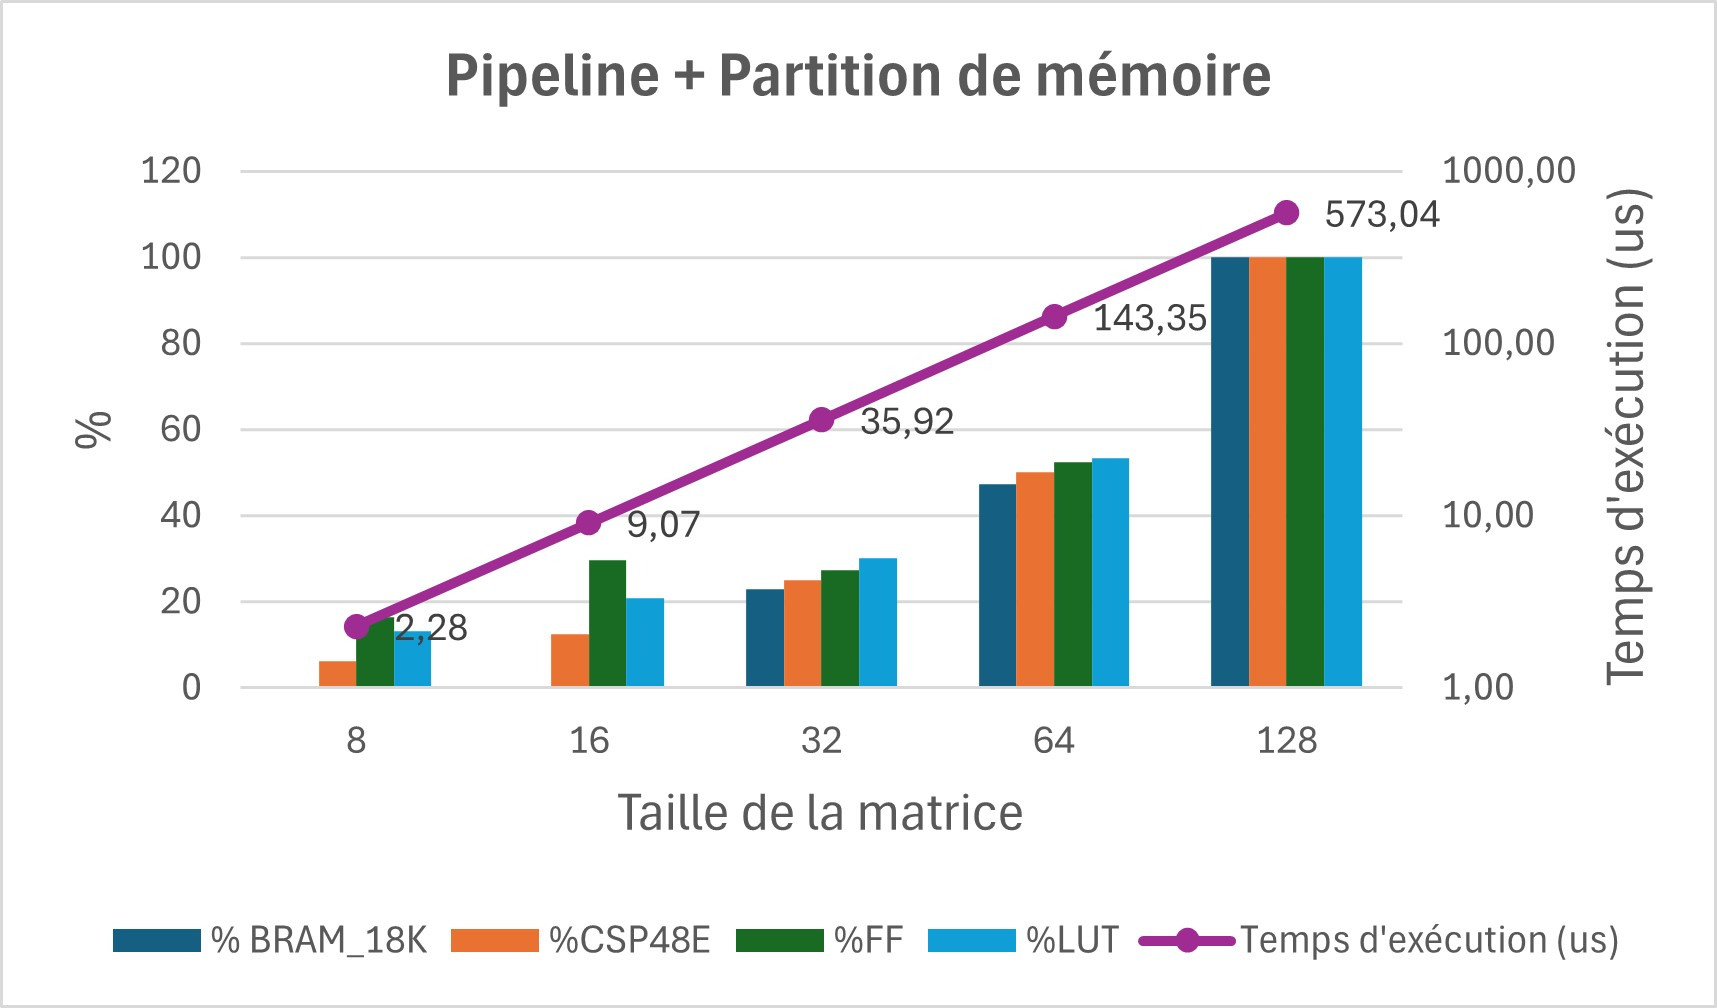
\includegraphics[width=1\columnwidth]{Images/Naive_2.jpg}
    \caption{Naïve avec partitionnement de pipelines et de tableaux.}
    \label{fig:3}
\end{figure}

Une grande amélioration des temps d’exécution est observée, mais au prix d’une utilisation considérable des ressources, notamment BRAM et CSP48E. Cela indique une plus grande parallélisation, ce qui augmente considérablement les performances. Cependant, la consommation de ressources est bien plus élevée.

\begin{figure}[H]
    \centering
    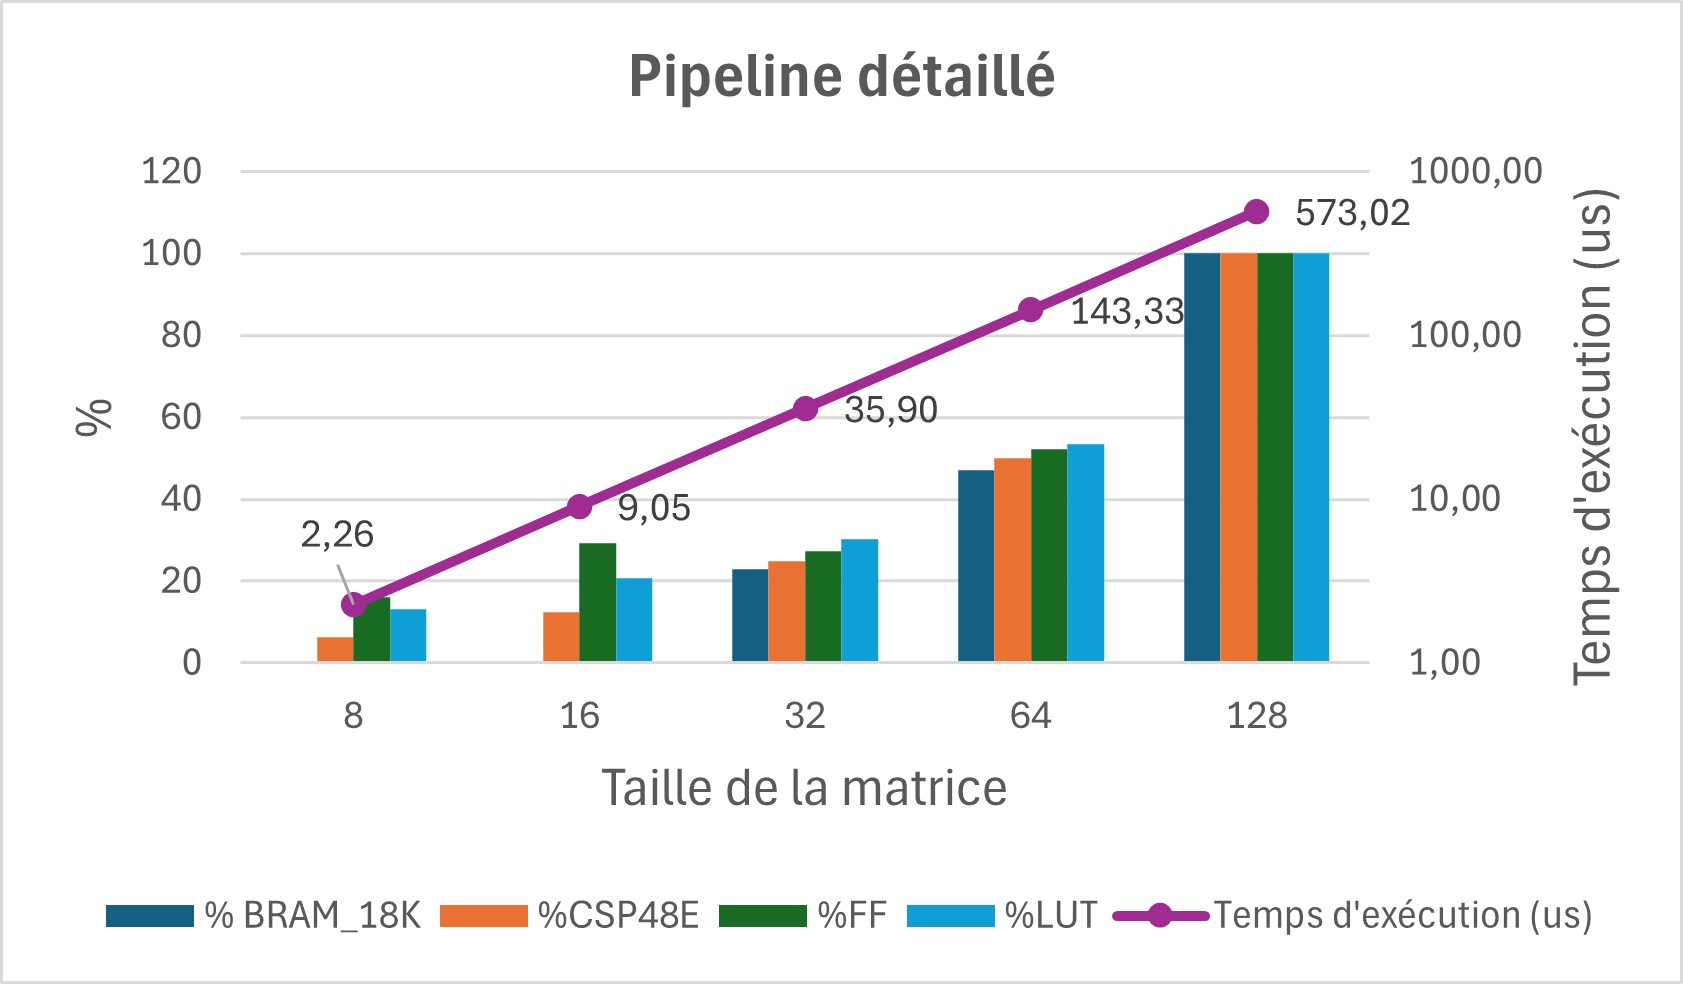
\includegraphics[width=1\columnwidth]{Images/Naive_3.jpg}
    \caption{Naïve avec pipeline détaillé.}
    \label{fig:4}
\end{figure}

Cette optimisation présente des temps d'exécution très similaires à ceux de la solution précédente, mais avec une utilisation légèrement plus efficace des bascules et des LUT. Cela suggère que le *rewind* est efficace pour améliorer la réutilisation des données sans avoir un impact important sur l'utilisation des ressources. Cependant, les bénéfices ne sont pas aussi significatifs par rapport à l’optimisation précédente.


L'optimisation (première optimisation) offre un bon compromis entre temps d'exécution et utilisation des ressources, tandis que les optimisations plus avancées (optimisation 2 et 3) sont utiles pour rechercher des performances maximales quelle que soit la consommation matérielle. Les améliorations des temps d'exécution s'accompagnent d'une augmentation considérable de l'utilisation de BRAM et d'autres ressources clés, qui doivent être évaluées en fonction des limites du FPGA.

L'utilisation de ressources de la carte est dans le cas Naïve pour la taille de matrice de 128 par 128 est présent ci-dessous:
\begin{figure}[H]
    \centering
    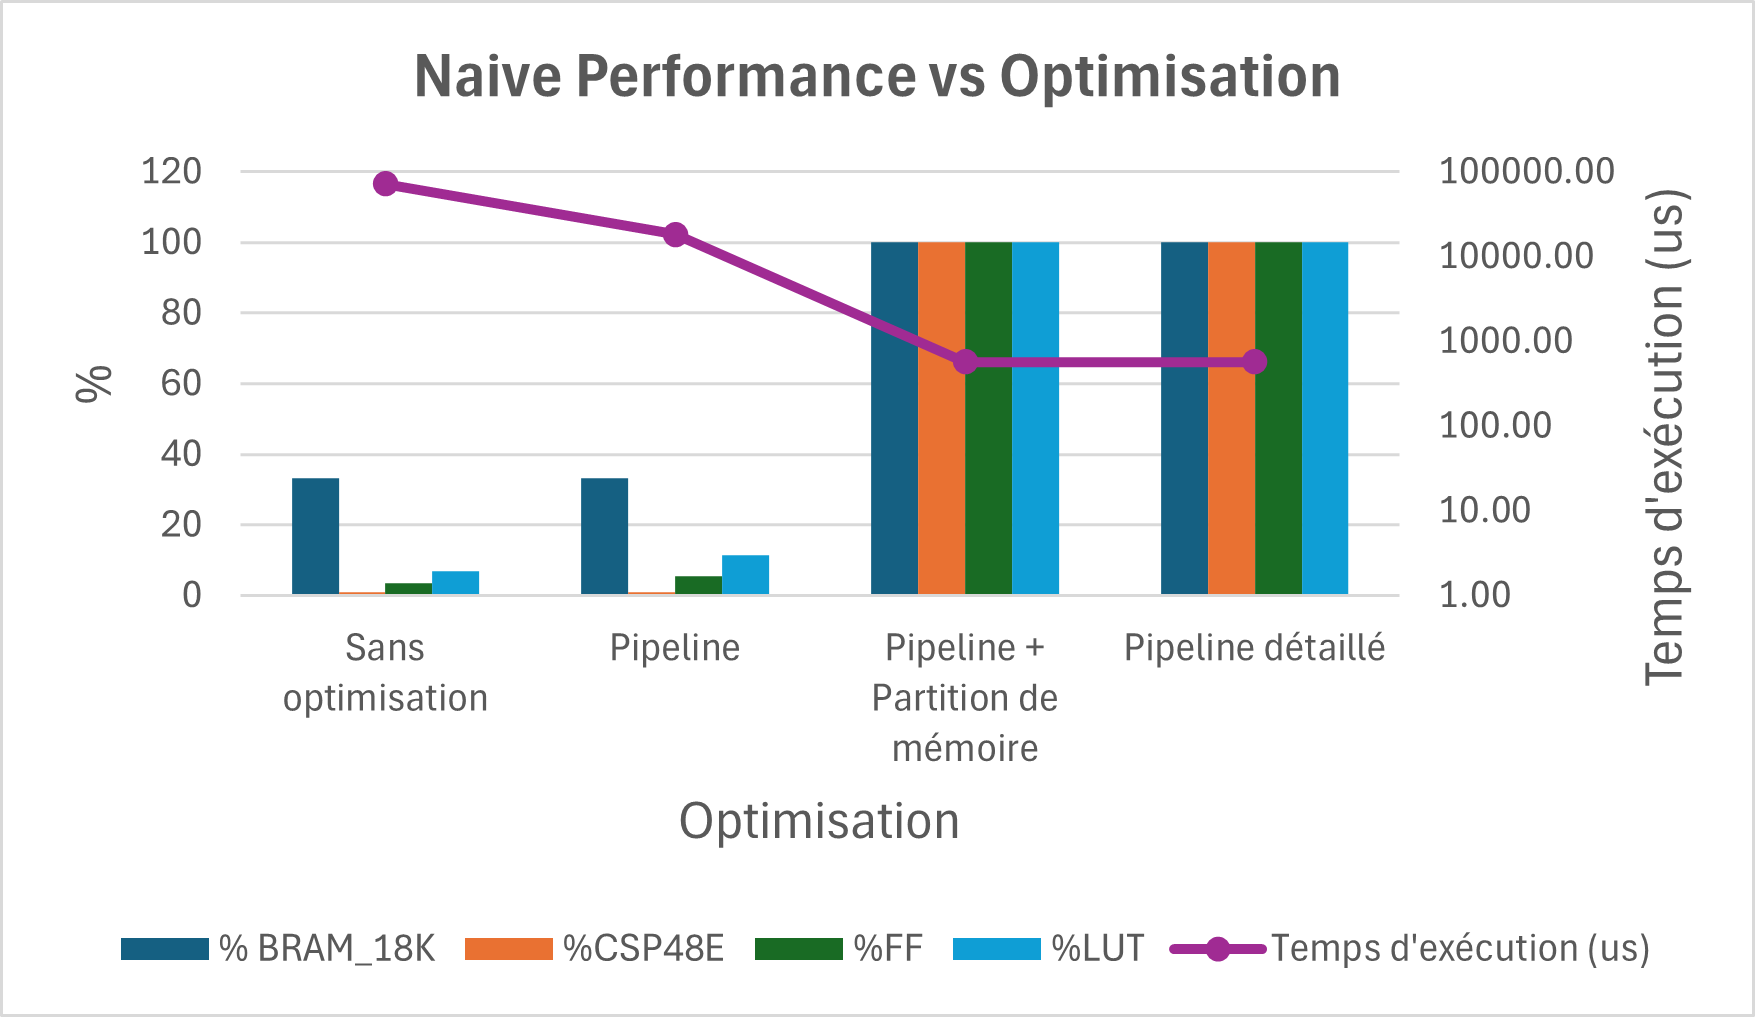
\includegraphics[width=1\columnwidth]{Images/naive_performance.png}
    \caption{Naïve performance par Optimisation.}
    \label{fig:4}
\end{figure}
L'utilisation du pipeline rend l'opération de multiplication de matrices plus efficace, mais utilise davantage de ressources. Ce comportement est également observé sur d'autres algorithmes à différentes échelles. Certains algorithmes, comme celui-ci, présentent une utilisation des ressources supérieure à ce qui est disponible sur le FPGA, rendant le circuit infaisable.



\subsection{Algorithme naïve réordonné}

\begin{figure}[H]
    \centering
    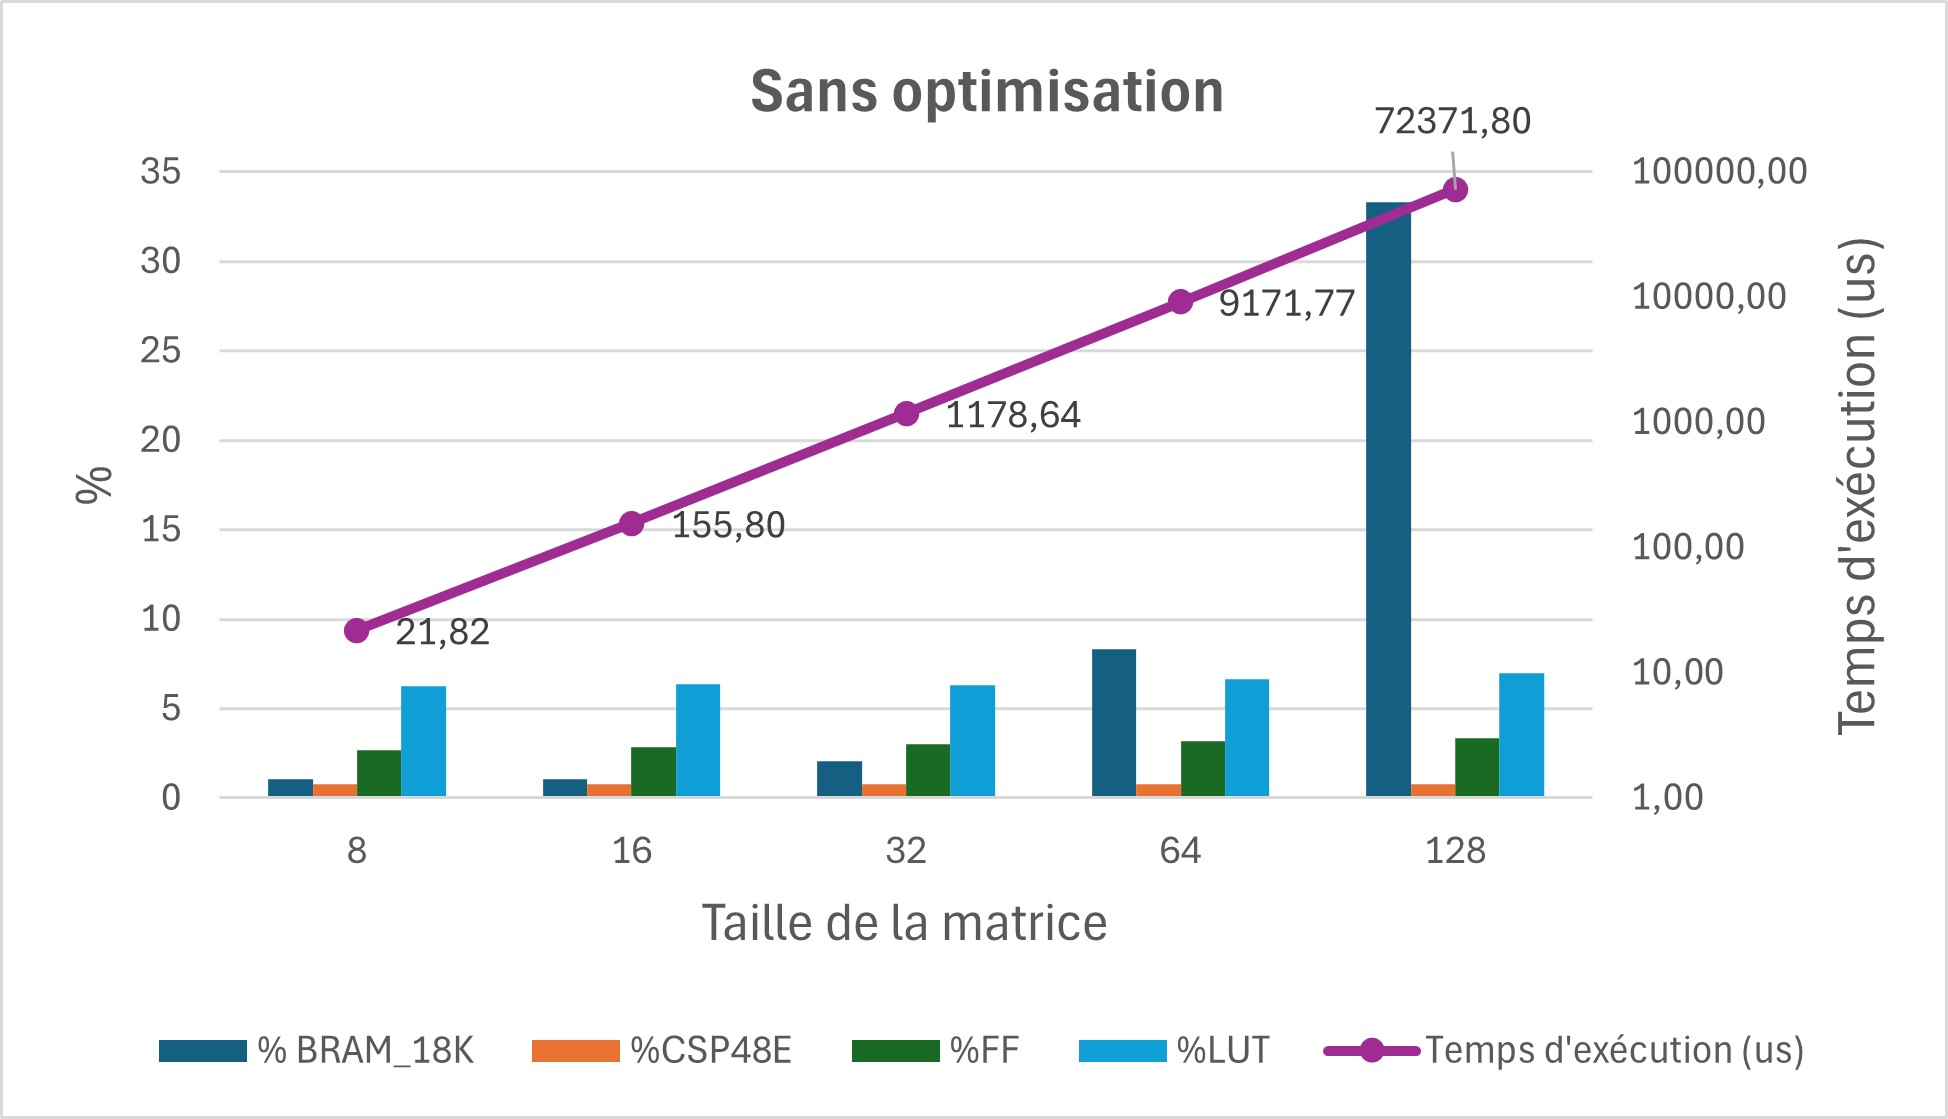
\includegraphics[width=1\columnwidth]{Images/Naive_R_0.jpg}
    \caption{Naïve Réordonné sans optimisation.}
    \label{fig:5}
\end{figure}

Le comportement est similaire à Naive sans optimisation. Les temps d'exécution sont très élevés pour les grandes matrices et l'utilisation des ressources est faible, ce qui indique une inefficacité de la multiplication sans optimisations.

\begin{figure}[H]
    \centering
    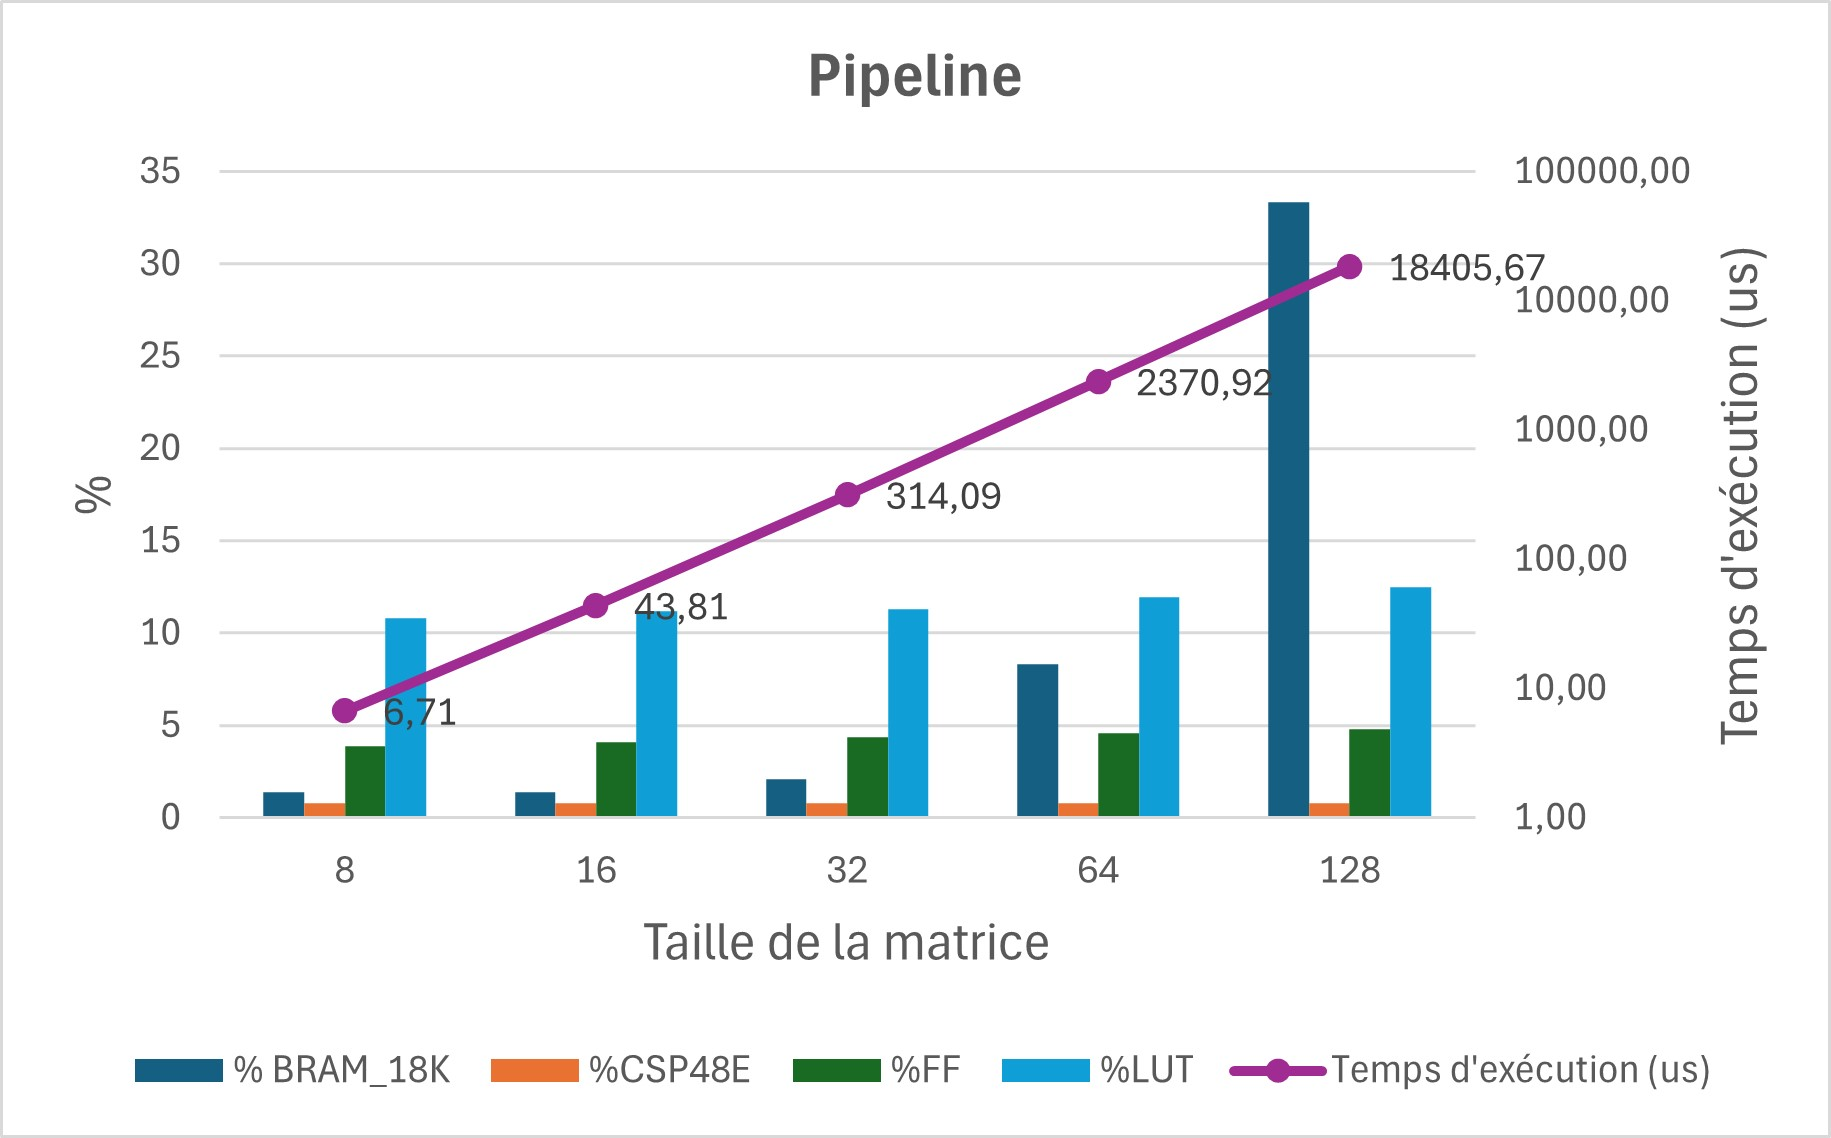
\includegraphics[width=1\columnwidth]{Images/Naive_R_1.jpg}
    \caption{Naïve Réordonné avec pipeline.}
    \label{fig:6}
\end{figure}

Le temps d'exécution est considérablement réduit, avec une utilisation modérée des ressources, améliorant les performances sans consommation matérielle excessive.

\begin{figure}[H]
    \centering
    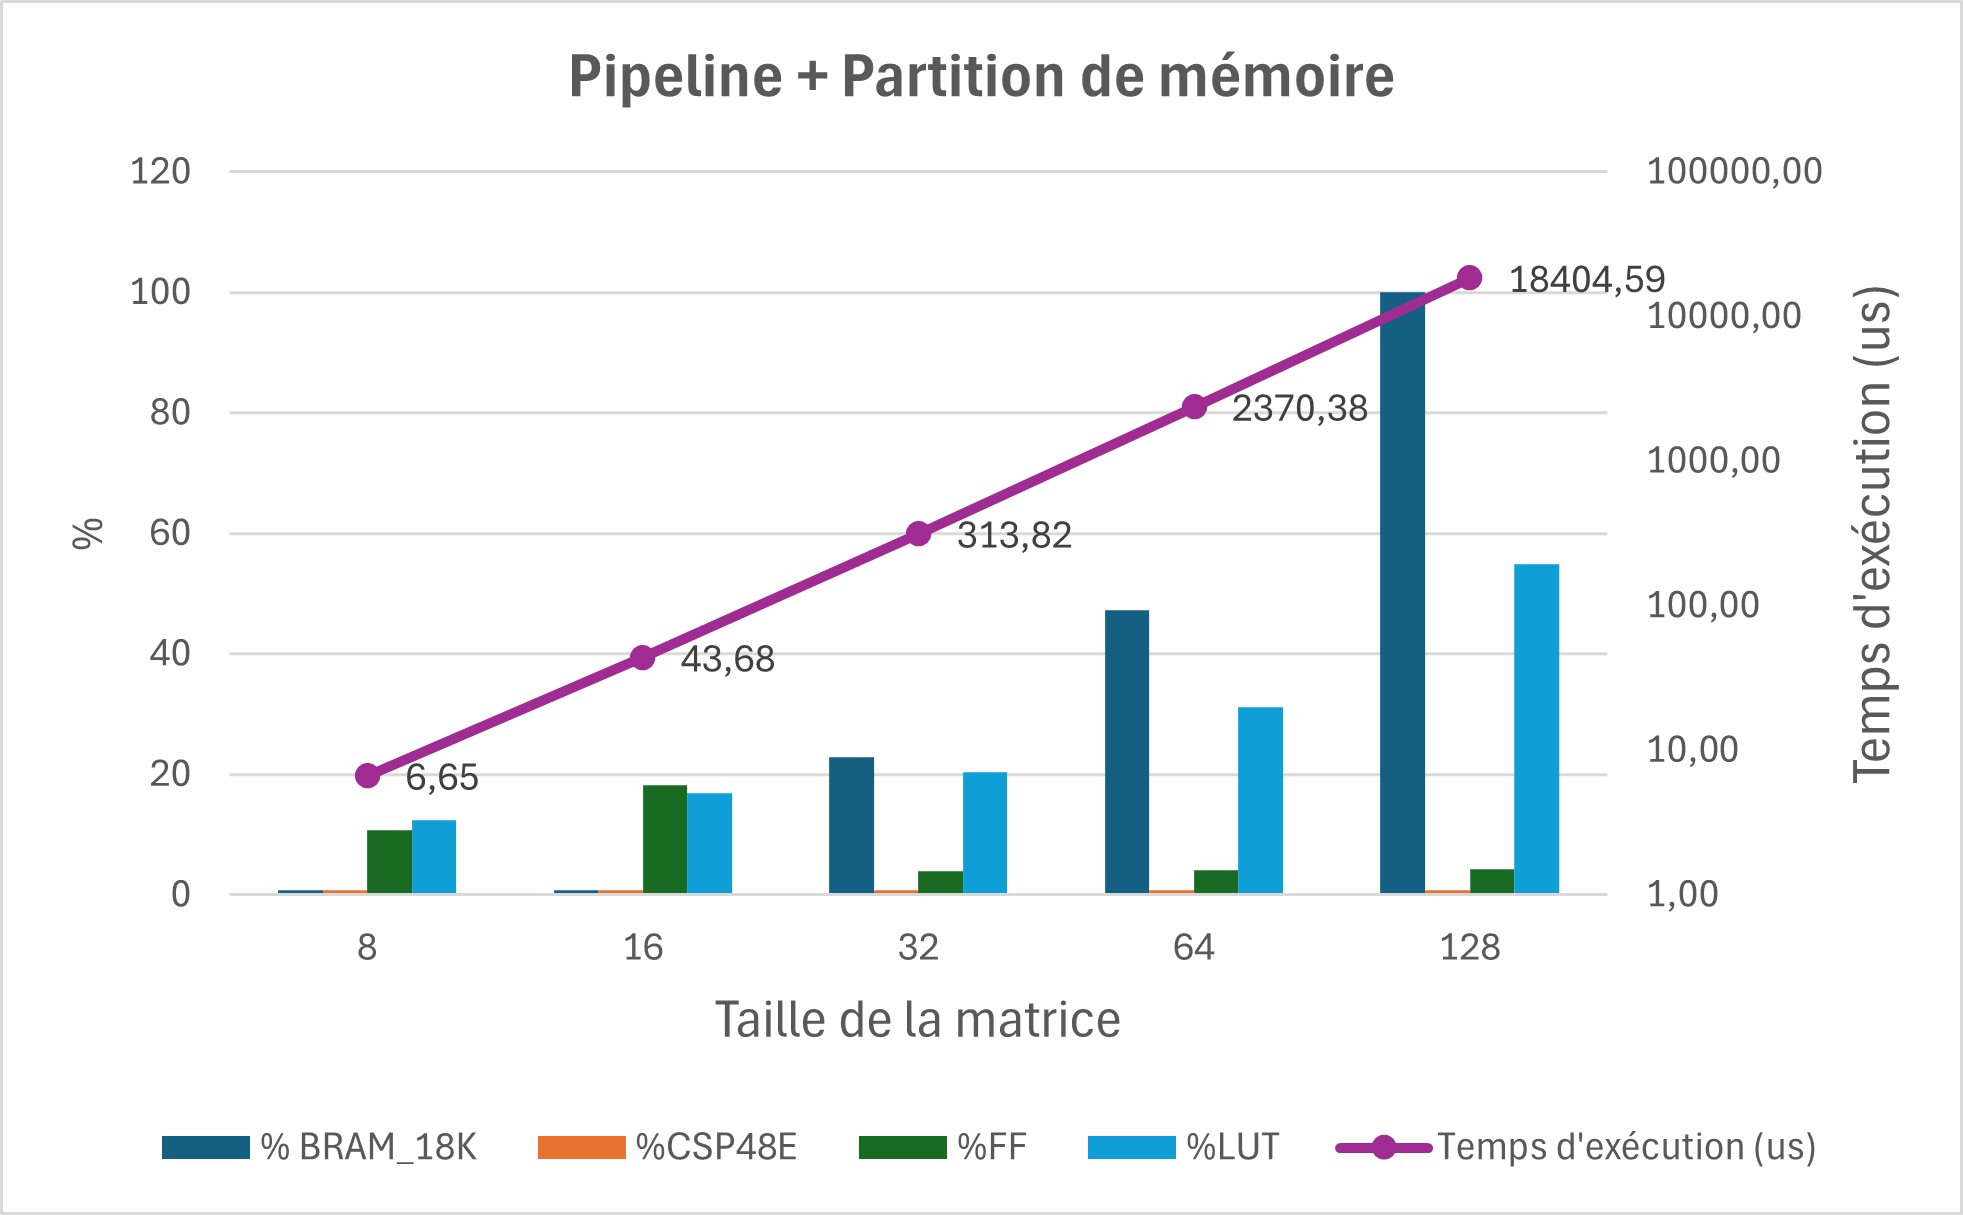
\includegraphics[width=1\columnwidth]{Images/Naive_R_2.jpg}
    \caption{Naïve Réordonné avec partitionnement de pipelines et de tableaux.}
    \label{fig:7}
\end{figure}

Le temps d'exécution reste quasiment le même, mais l'utilisation des ressources s'élèvent considérablement. Alors, nous comprenons que l'algorithme réordonné est modulé de façon qu'une routine additionnelle de partition de mémoire soit inefficace pour la multiplication de matrices.

\begin{figure}[H]
    \centering
    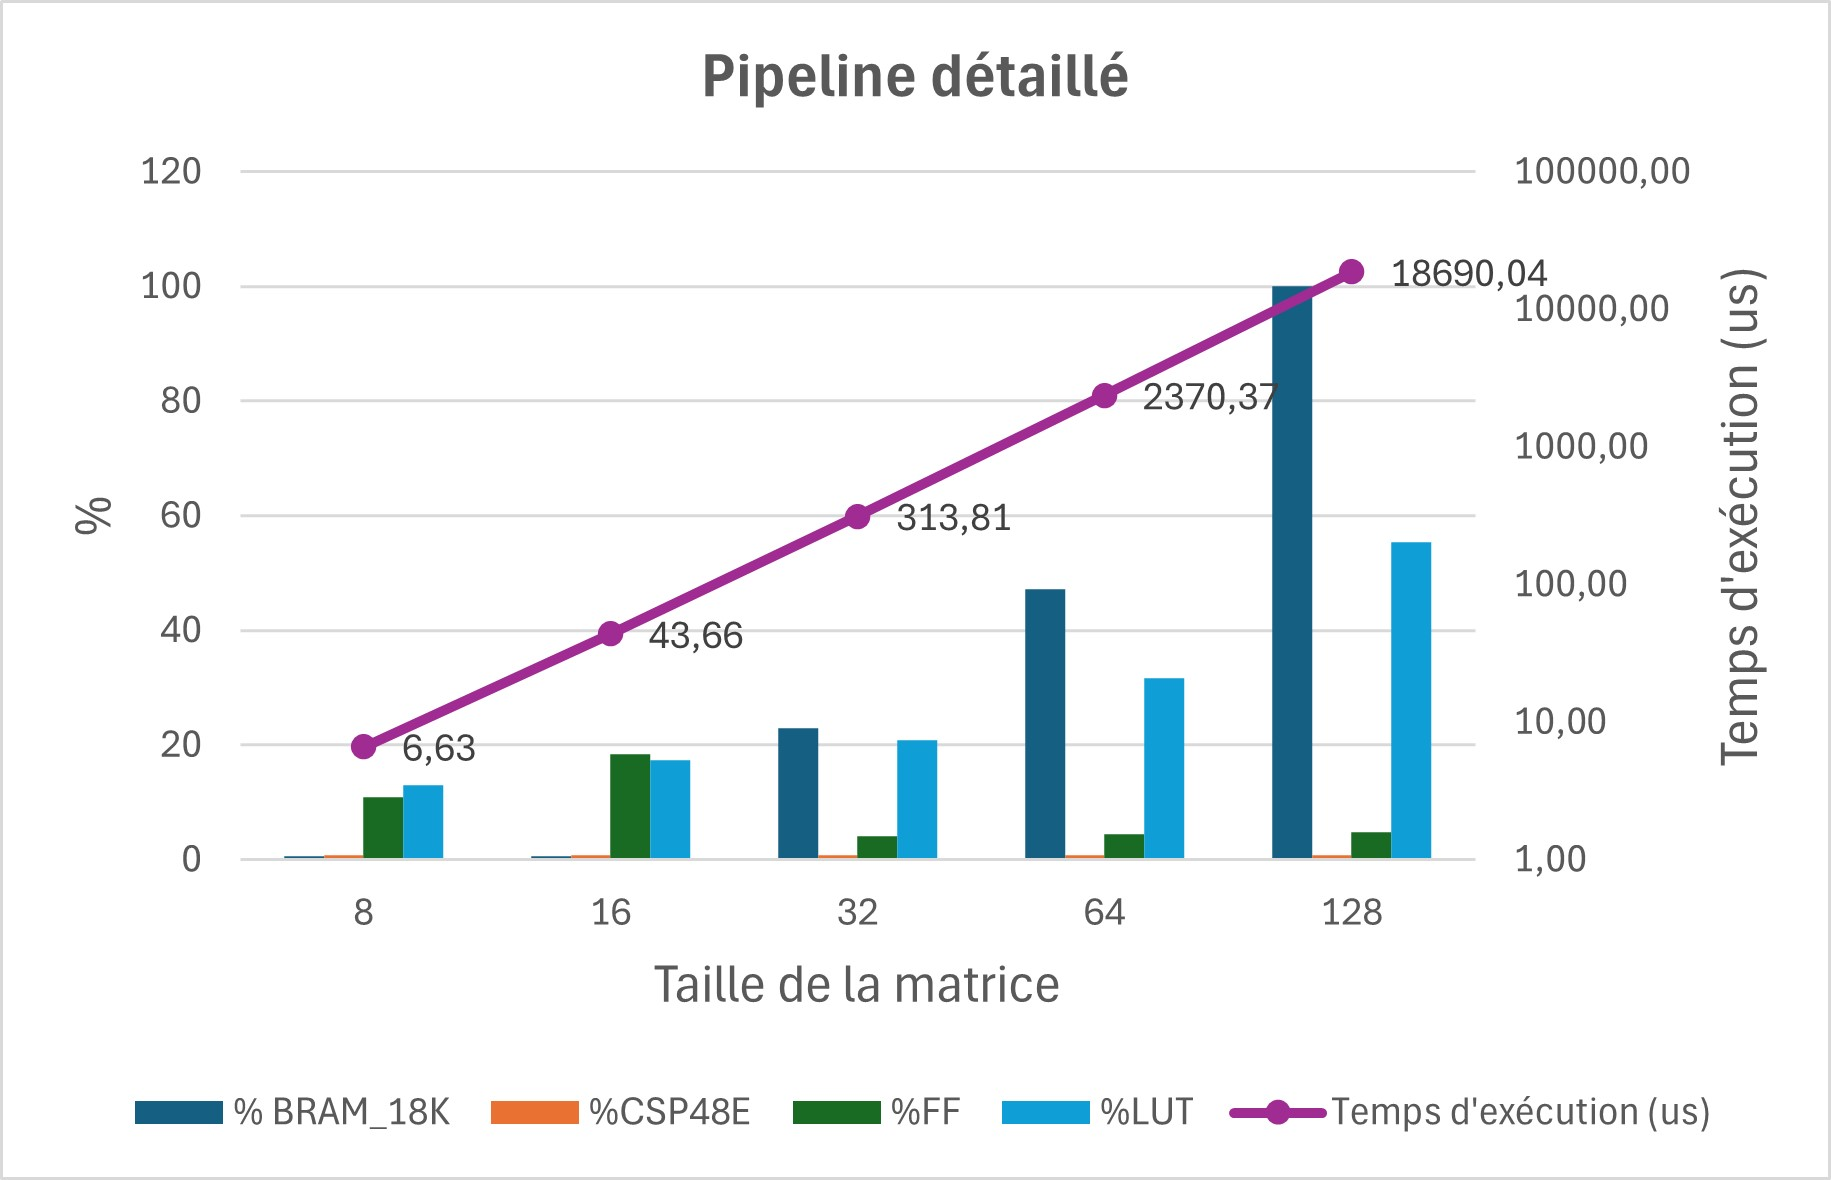
\includegraphics[width=1\columnwidth]{Images/Naive_R_3.jpg}
    \caption{Naïve Réordonné avec pipeline détaillé.}
    \label{fig:8}
\end{figure}

Des performances sont similaires à la solution précédente. Nous comprenons que cette optimisation aussi utilise des ressources inefficacement par rapport à la première pipeline.

\subsection{Algorithme des Blocs}

\begin{figure}[H]
    \centering
    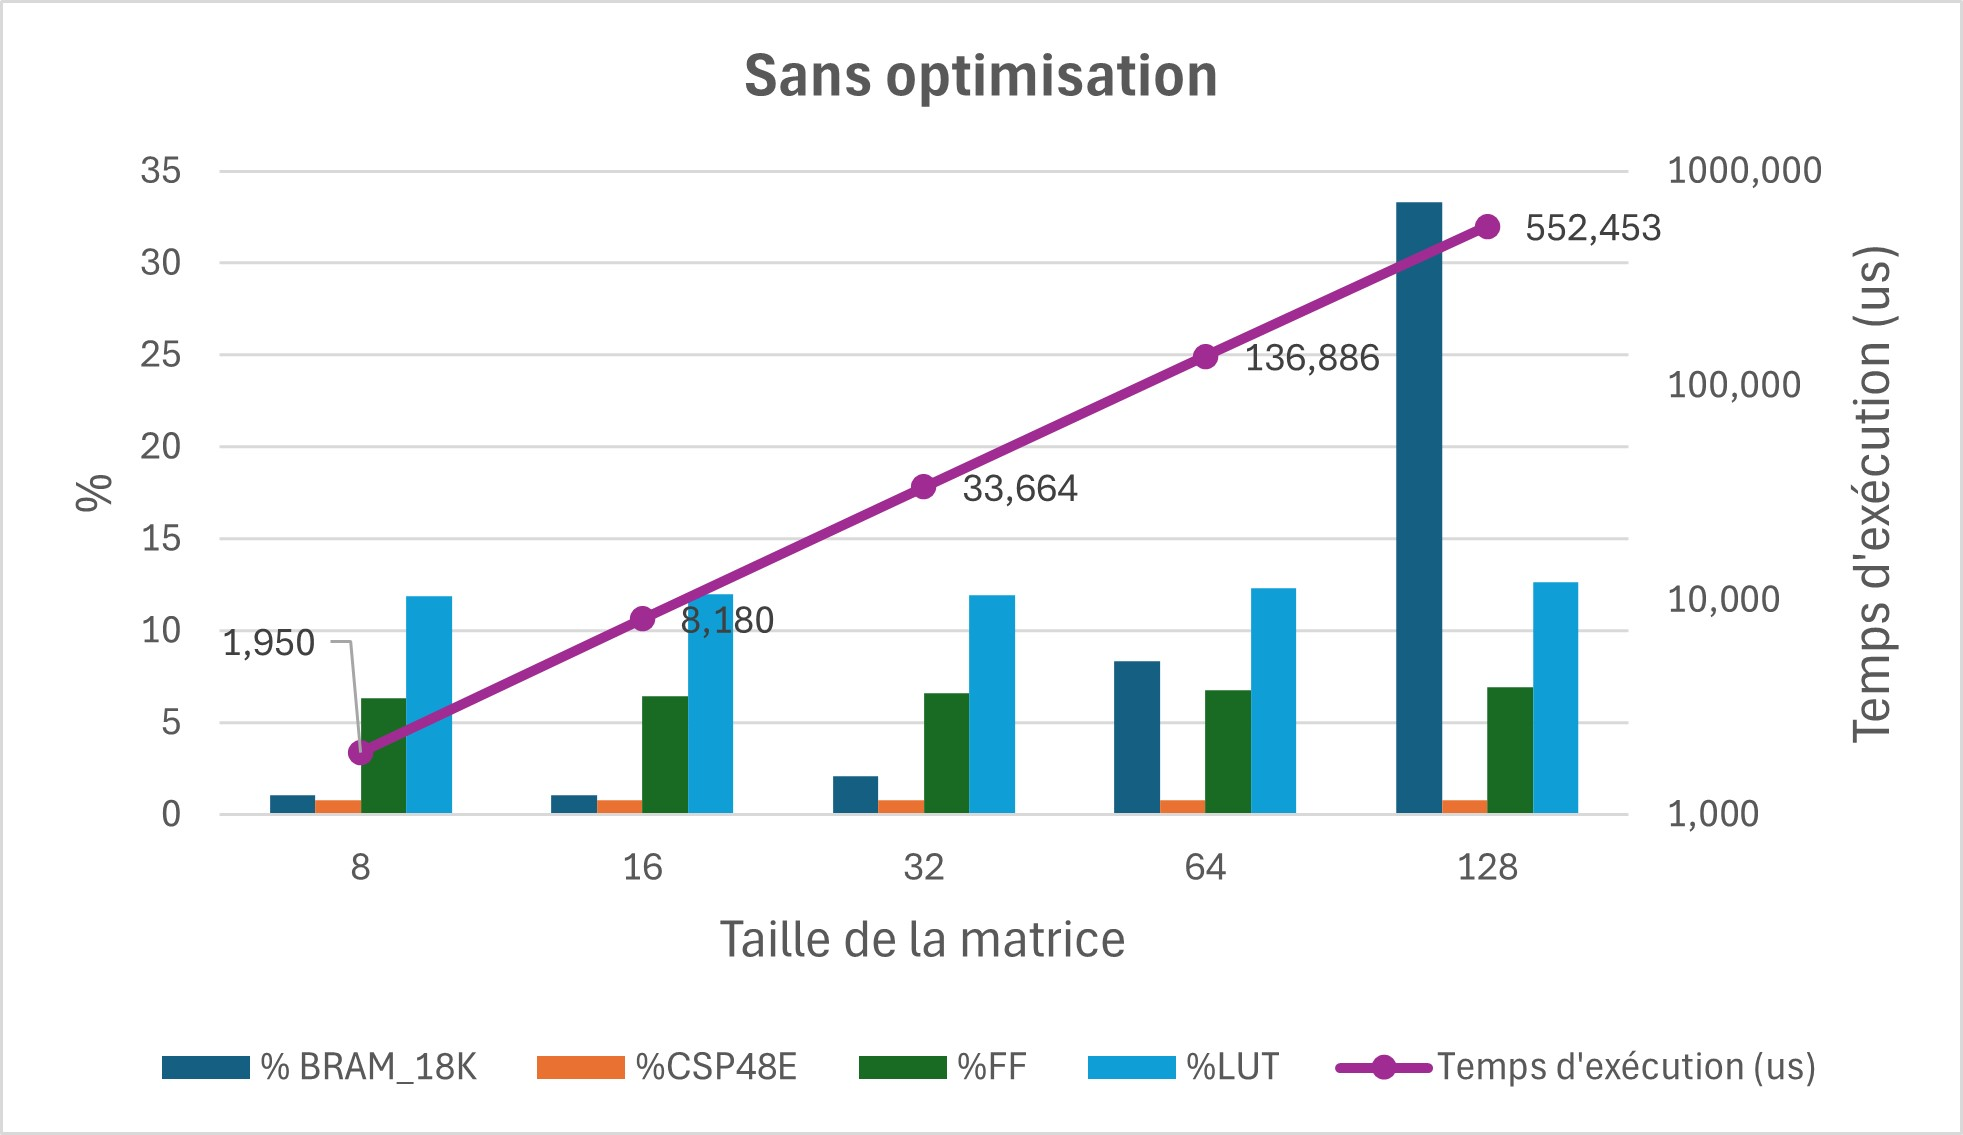
\includegraphics[width=1\columnwidth]{Images/Bloques_0.jpg}
    \caption{Blocs sans optimisation.}
    \label{fig:9}
\end{figure}

Les temps d’exécution sont extrêmement faibles par rapport à Naive, du fait de l’efficacité intrinsèque de la méthode par blocs. L'utilisation des ressources est minime, ce qui le rend idéal pour les petites baies, mais pourrait bénéficier d'optimisations pour améliorer encore les performances sur les grandes baies.

\begin{figure}[H]
    \centering
    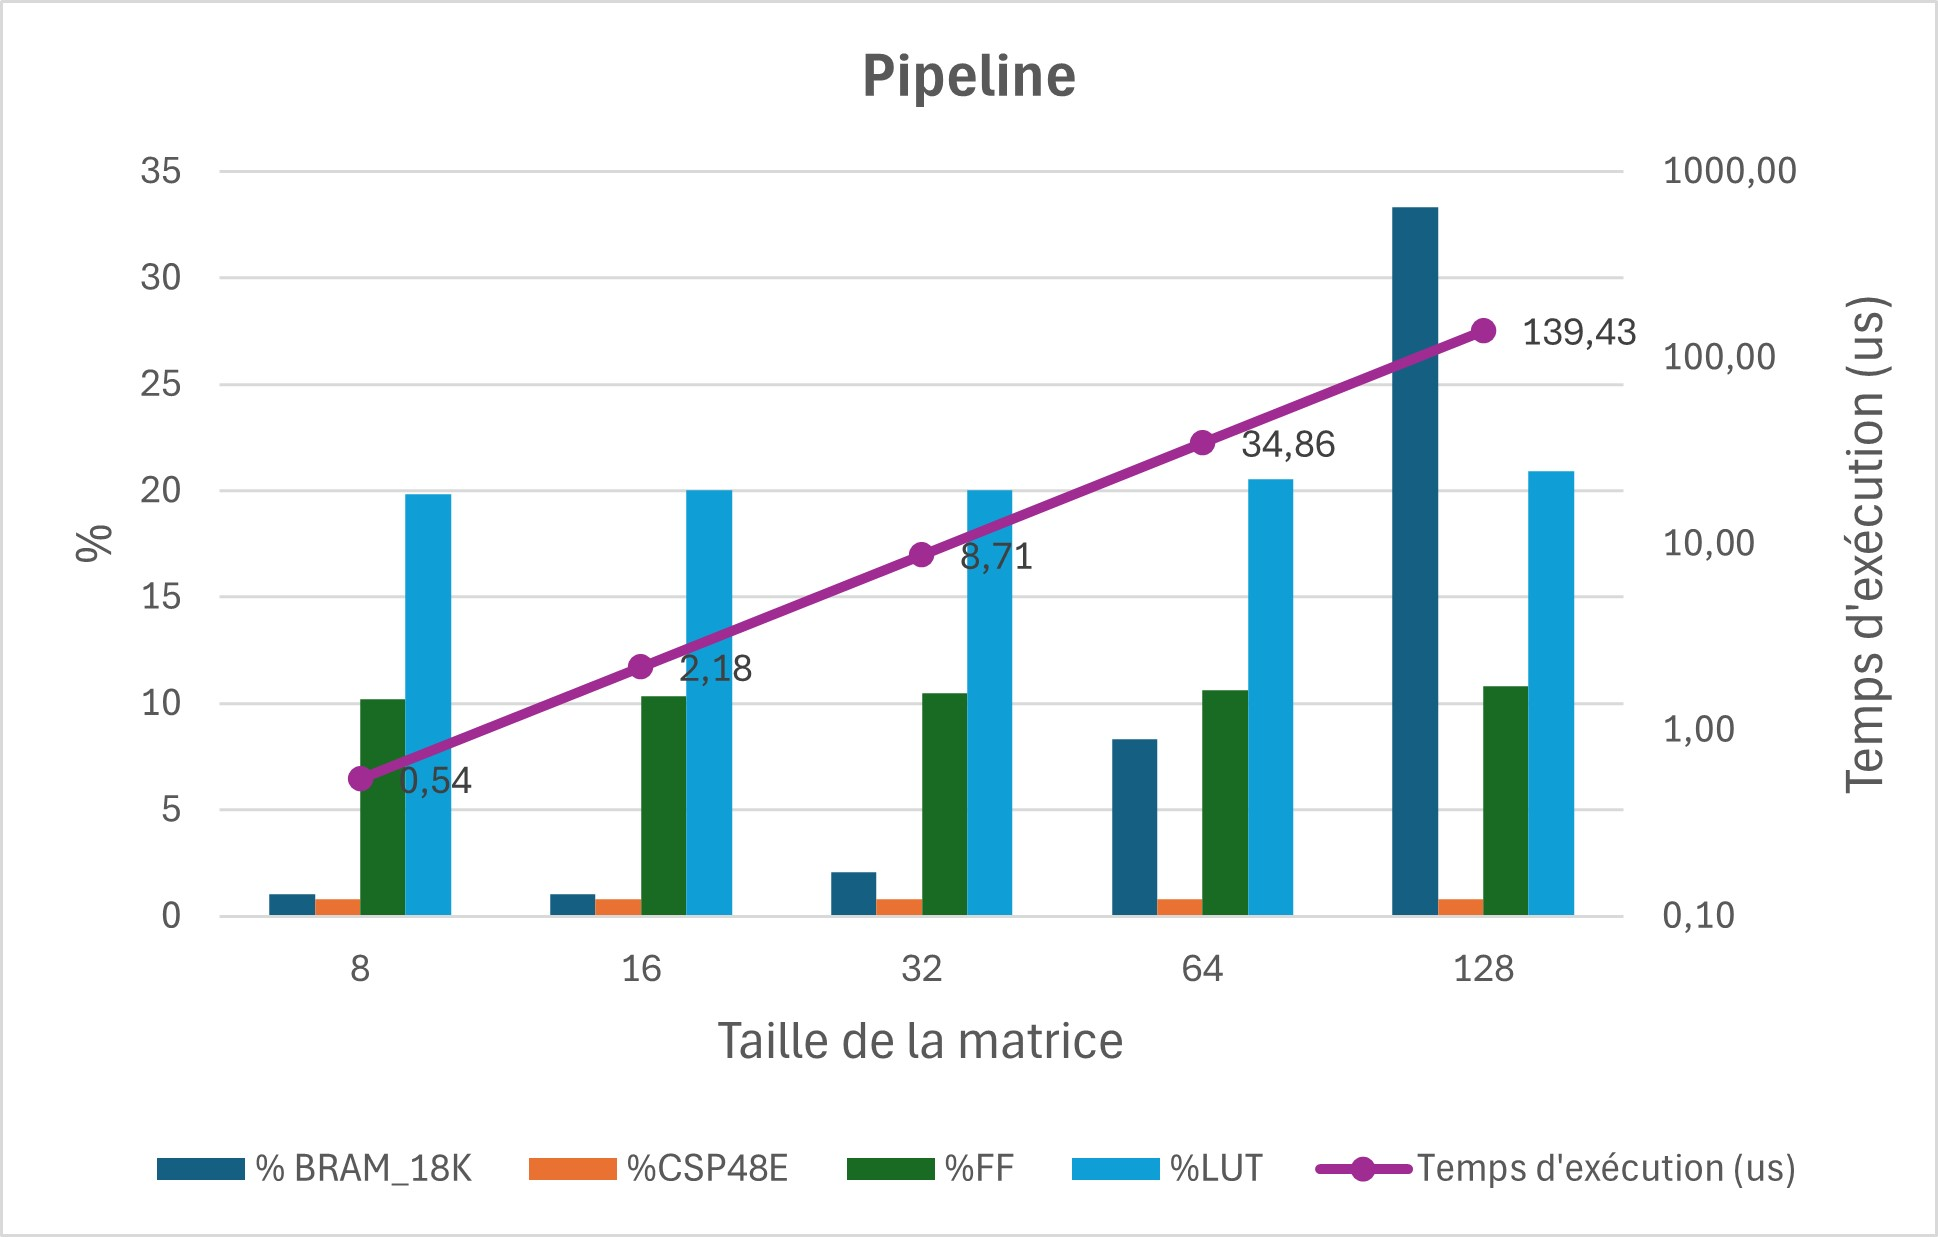
\includegraphics[width=1\columnwidth]{Images/Bloques_1.jpg}
    \caption{Blocs avec pipeline.}
    \label{fig:10}
\end{figure}

Le temps d'exécution diminue, et l'utilisation des ressources devient plus homogène avec différents tailles de tableau. La valeur \%FF est la seule qu'augmente considérablement avec la taille de matrices, mais est encore réduite en comparaison avec l'algorithme sans optimisation. Cette configuration indique un équilibre entre temps d'exécution et utilisation des ressources.

\begin{figure}[H]
    \centering
    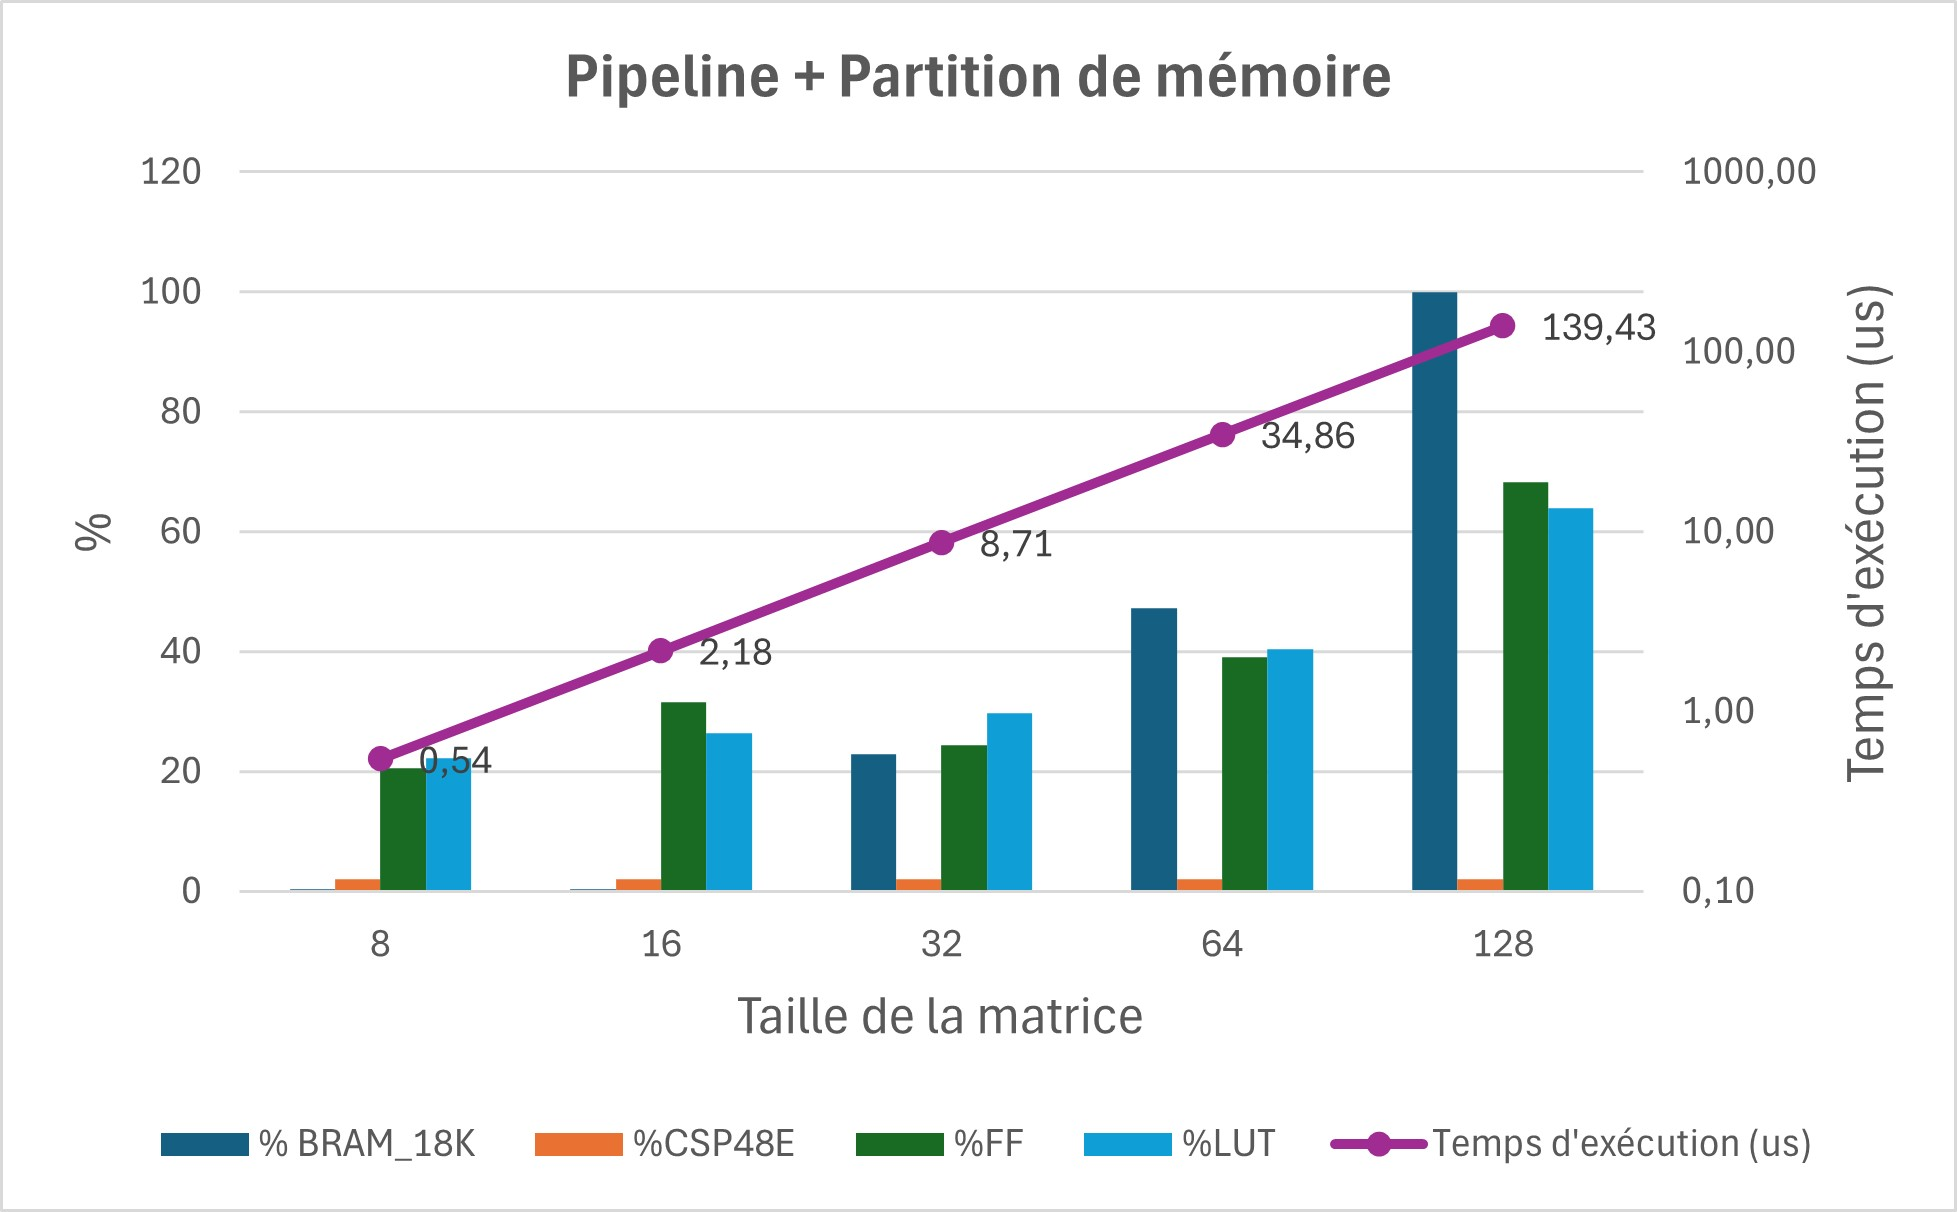
\includegraphics[width=1\columnwidth]{Images/Bloques_2.jpg}
    \caption{Blocs avec partitionnement de pipelines et de tableaux.}
    \label{fig:11}
\end{figure}

Il y a beaucoup plus d'utilisation de BRAM et FF, mais avec des temps d'exécution similaires à ceux de l'optimisation précédente. Ceci suggère que cette configuration consomme plus de ressources sans amélioration significative du temps d'exécution.

\begin{figure}[H]
    \centering
    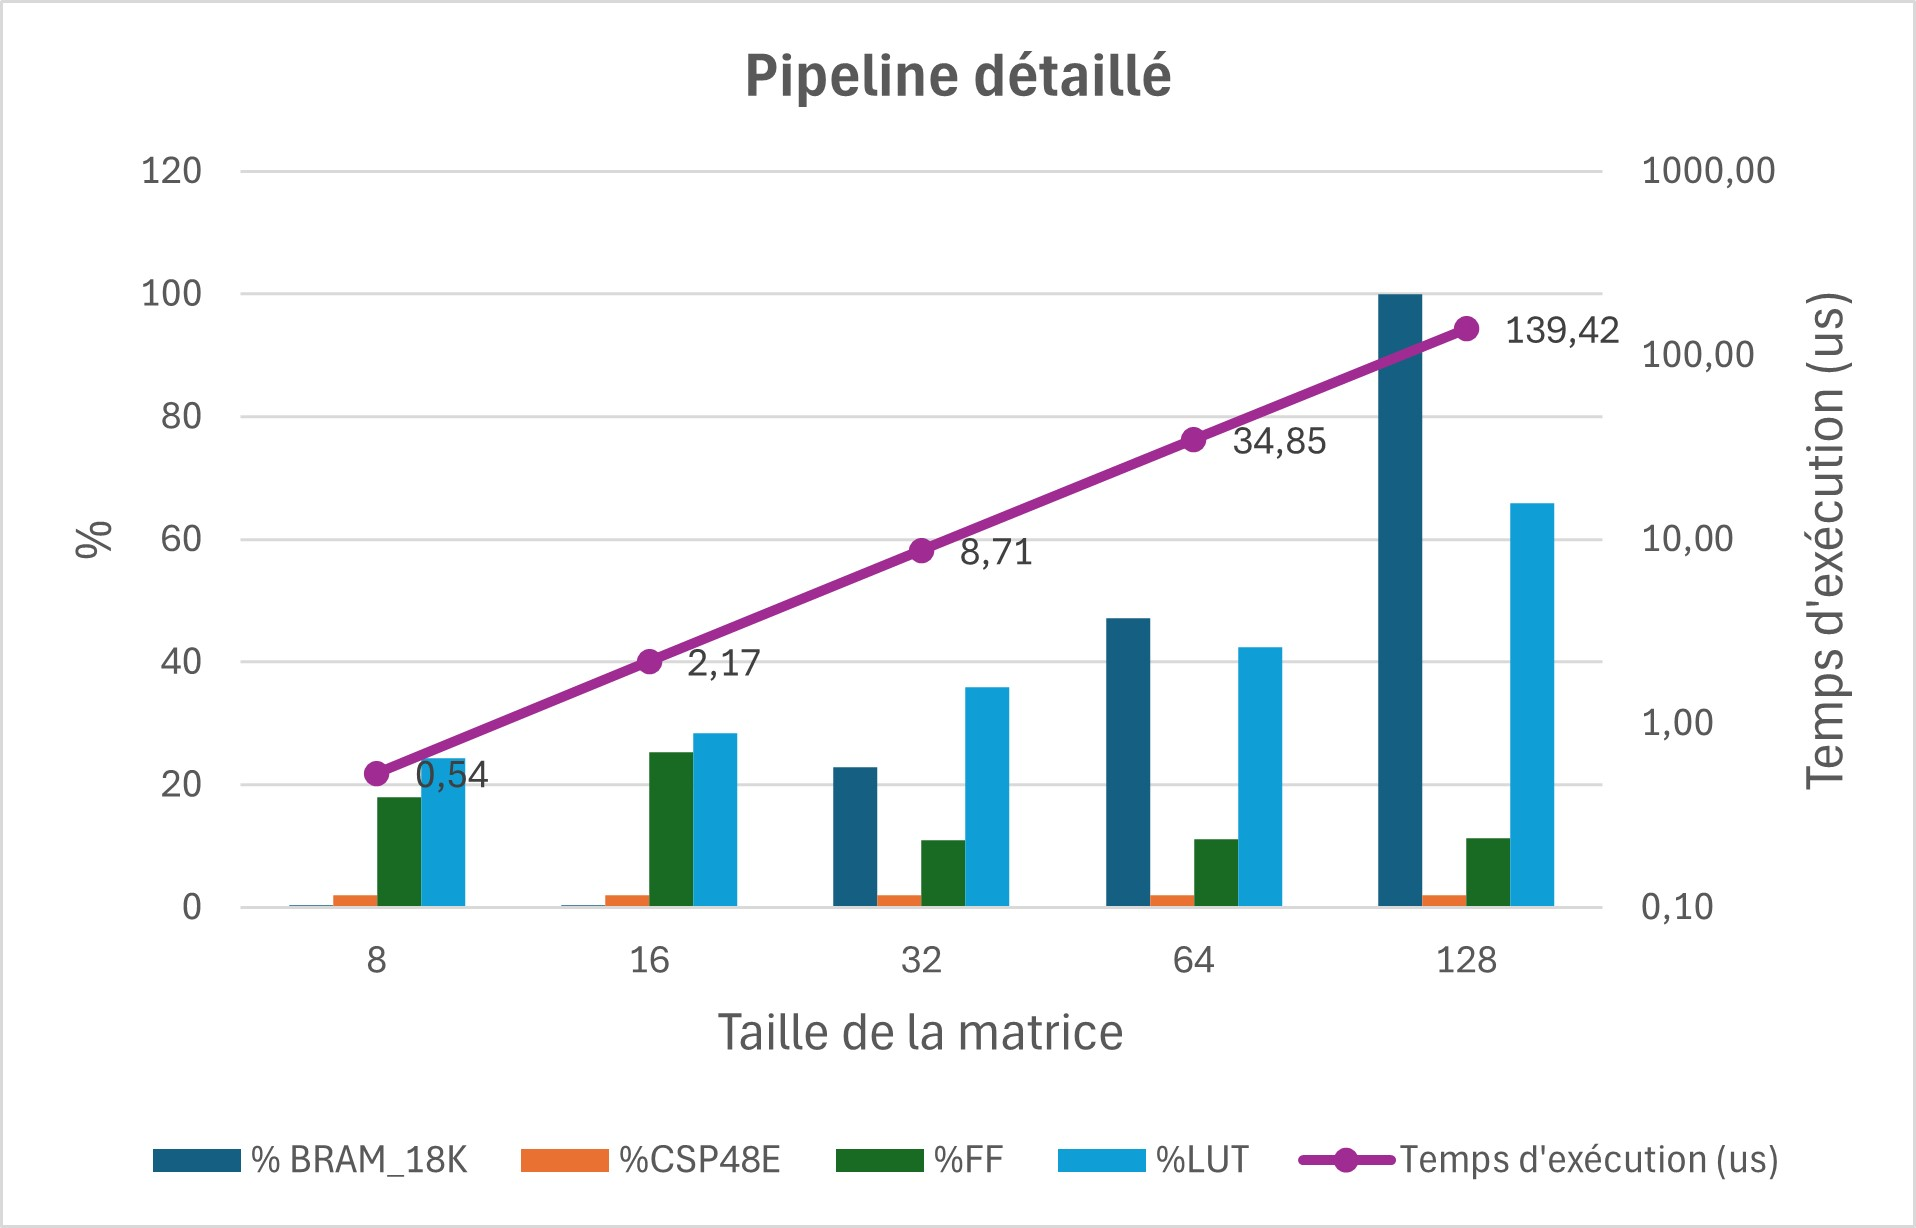
\includegraphics[width=1\columnwidth]{Images/Bloques_3.jpg}
    \caption{Blocs avec pipeline détaillé.}
    \label{fig:12}
\end{figure}


Les performances sont pratiquement les mêmes que celles de la solution de baie partitionnée. Cela augmente légèrement l'utilisation des ressources, mais il n'y a pas de grandes différences dans les temps d'exécution.

La multiplication de blocs est nettement plus efficace en termes de temps d'exécution par rapport à Naive, notamment sur les petites matrices. Cependant, les optimisations introduisent une utilisation plus élevée des ressources (FF, LUT, BRAM) sans amélioration drastique des temps d'exécution, notamment dans les configurations plus avancées telles que le partitionnement des baies. Cela suggère que pour certaines applications, la solution sans optimisation pourrait être plus adaptée si une utilisation réduite du matériel est prioritaire.


\subsection{Algorithme des Blocs réordonné}

\begin{figure}[H]
    \centering
    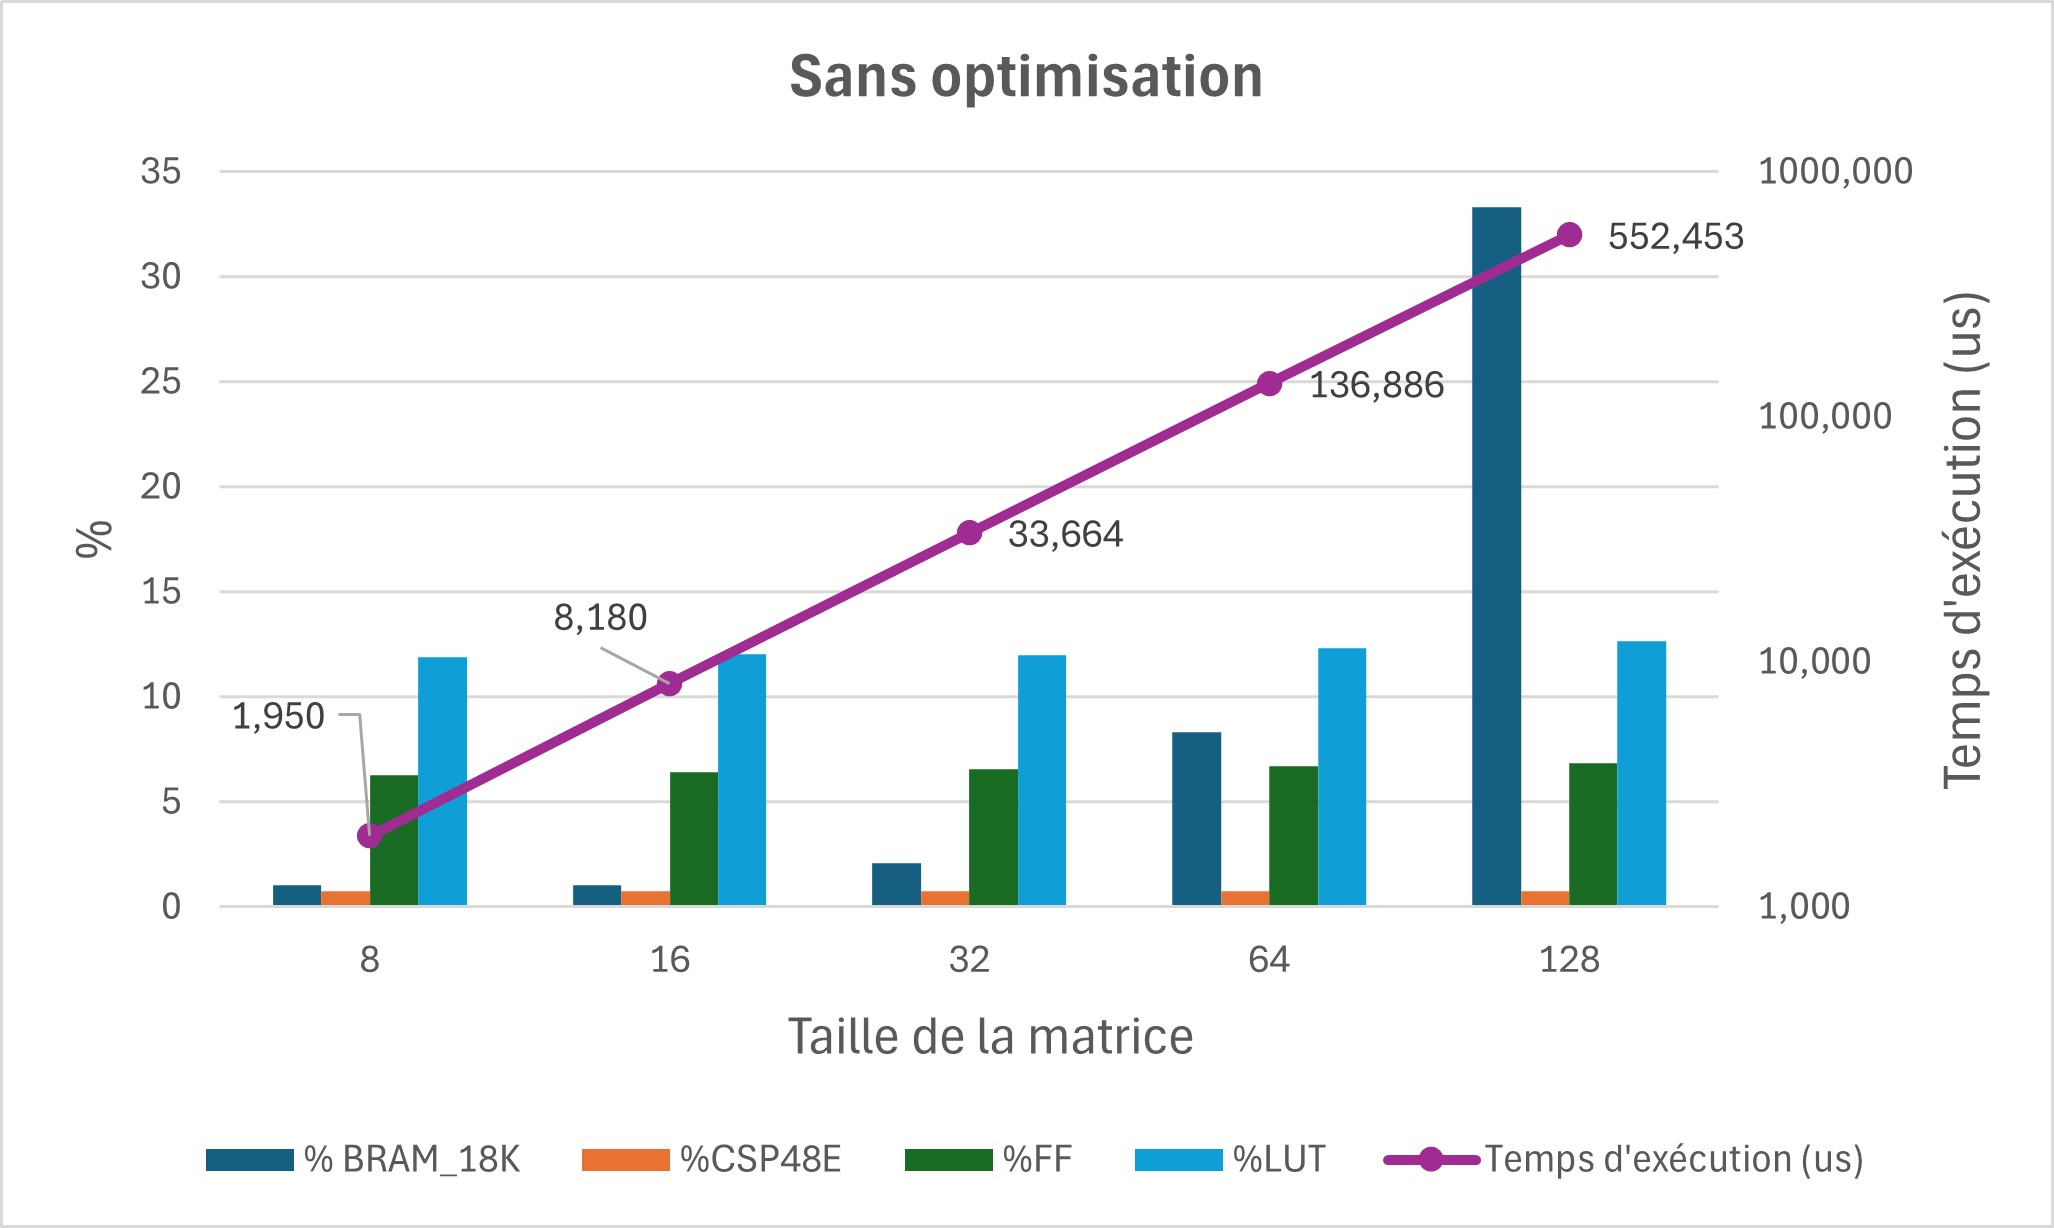
\includegraphics[width=1\columnwidth]{Images/Bloques_R_0.jpg}
    \caption{Blocs Réordonné sans optimisation.}
    \label{fig:13}
\end{figure}

Il se comporte pratiquement de la même manière que la version non réorganisée, ce qui suggère que la réorganisation n'affecte pas de manière significative les petits tableaux.

\begin{figure}[H]
    \centering
    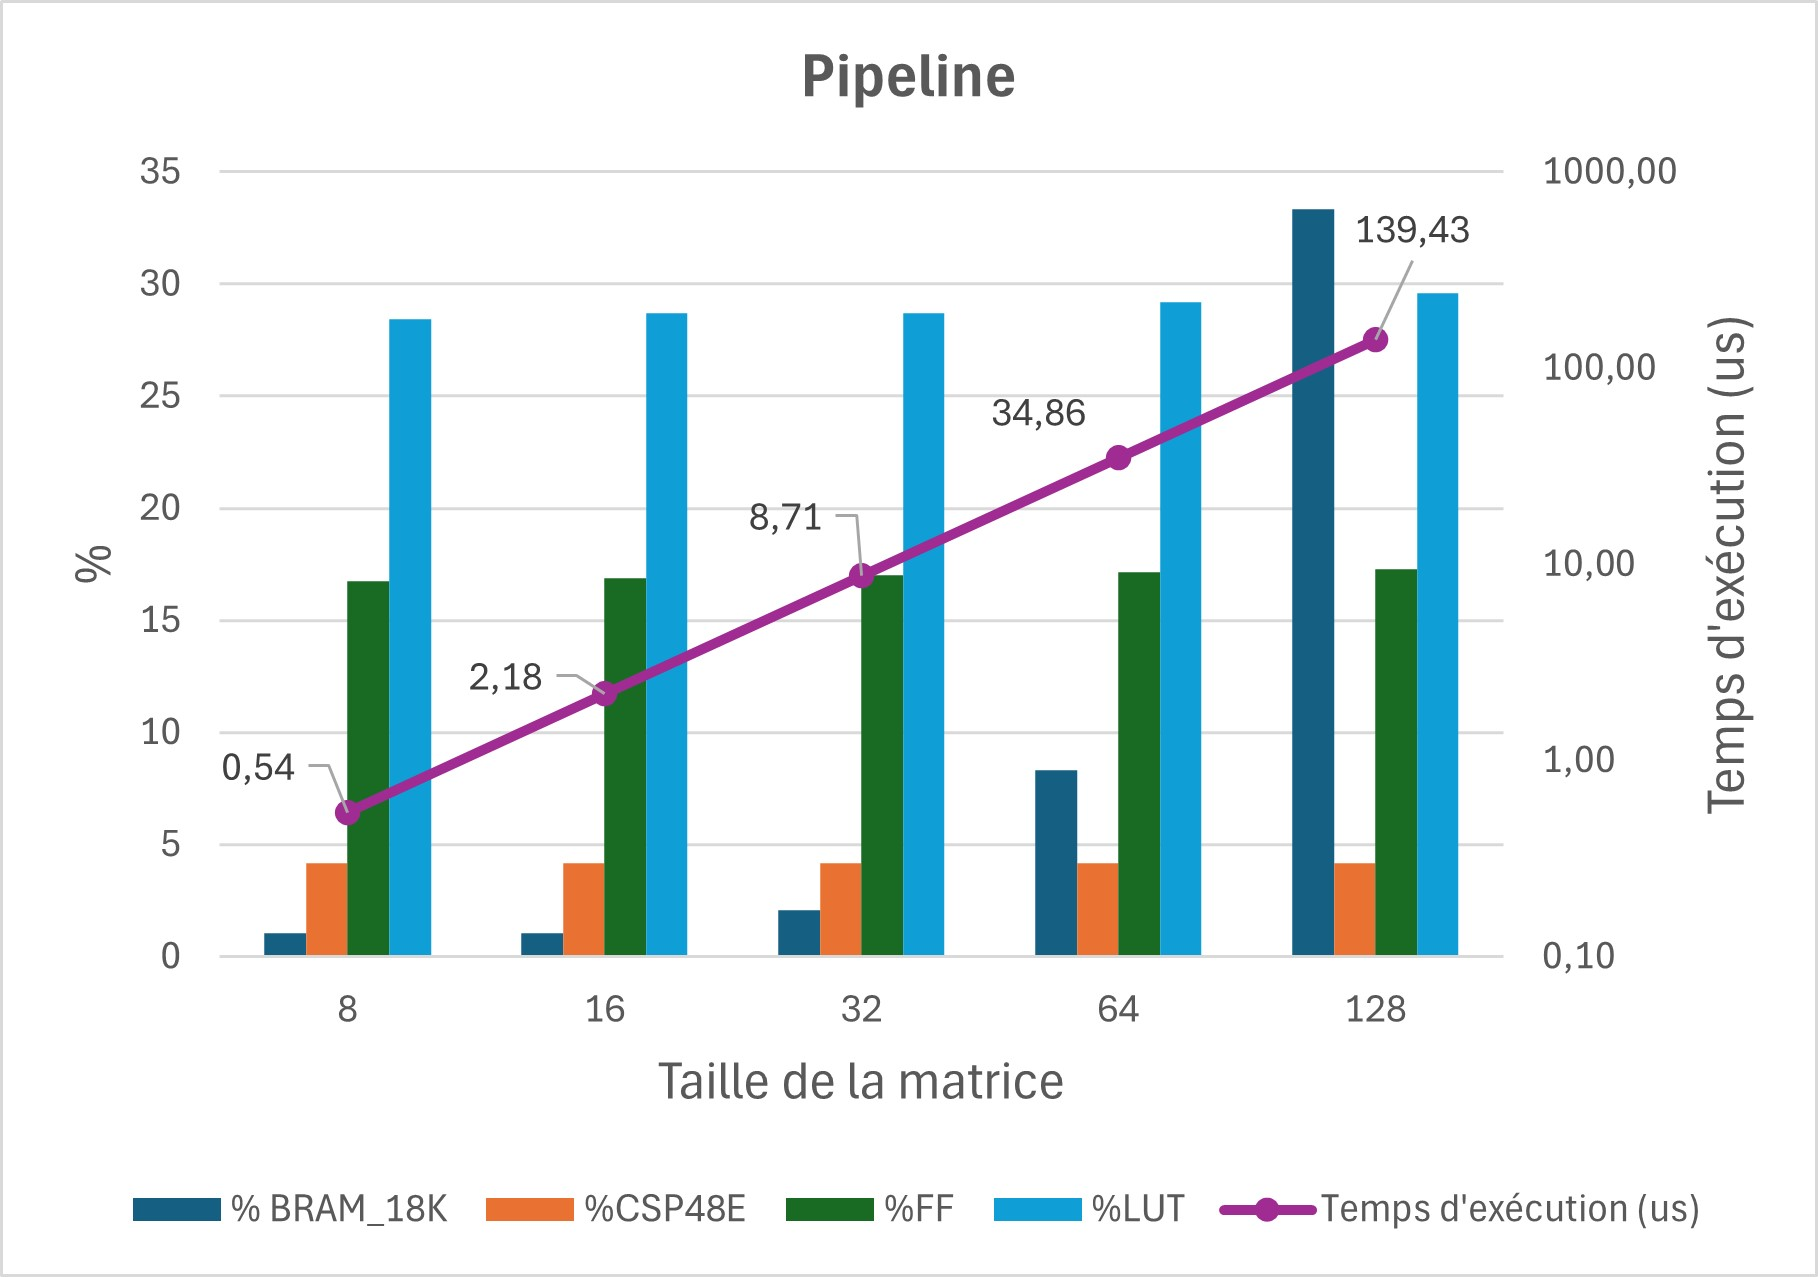
\includegraphics[width=1\columnwidth]{Images/Bloques_R_1.jpg}
    \caption{Blocs Réordonné avec pipeline.}
    \label{fig:14}
\end{figure}

Cela augmente légèrement l'utilisation des ressources par rapport à la version non réorganisée, mais les temps d'exécution est considérablement réduit. Alors, cette optimisation suggère que la réorganisation consomme plus de matériel sans gain de vitesse notable. 

\begin{figure}[H]
    \centering
    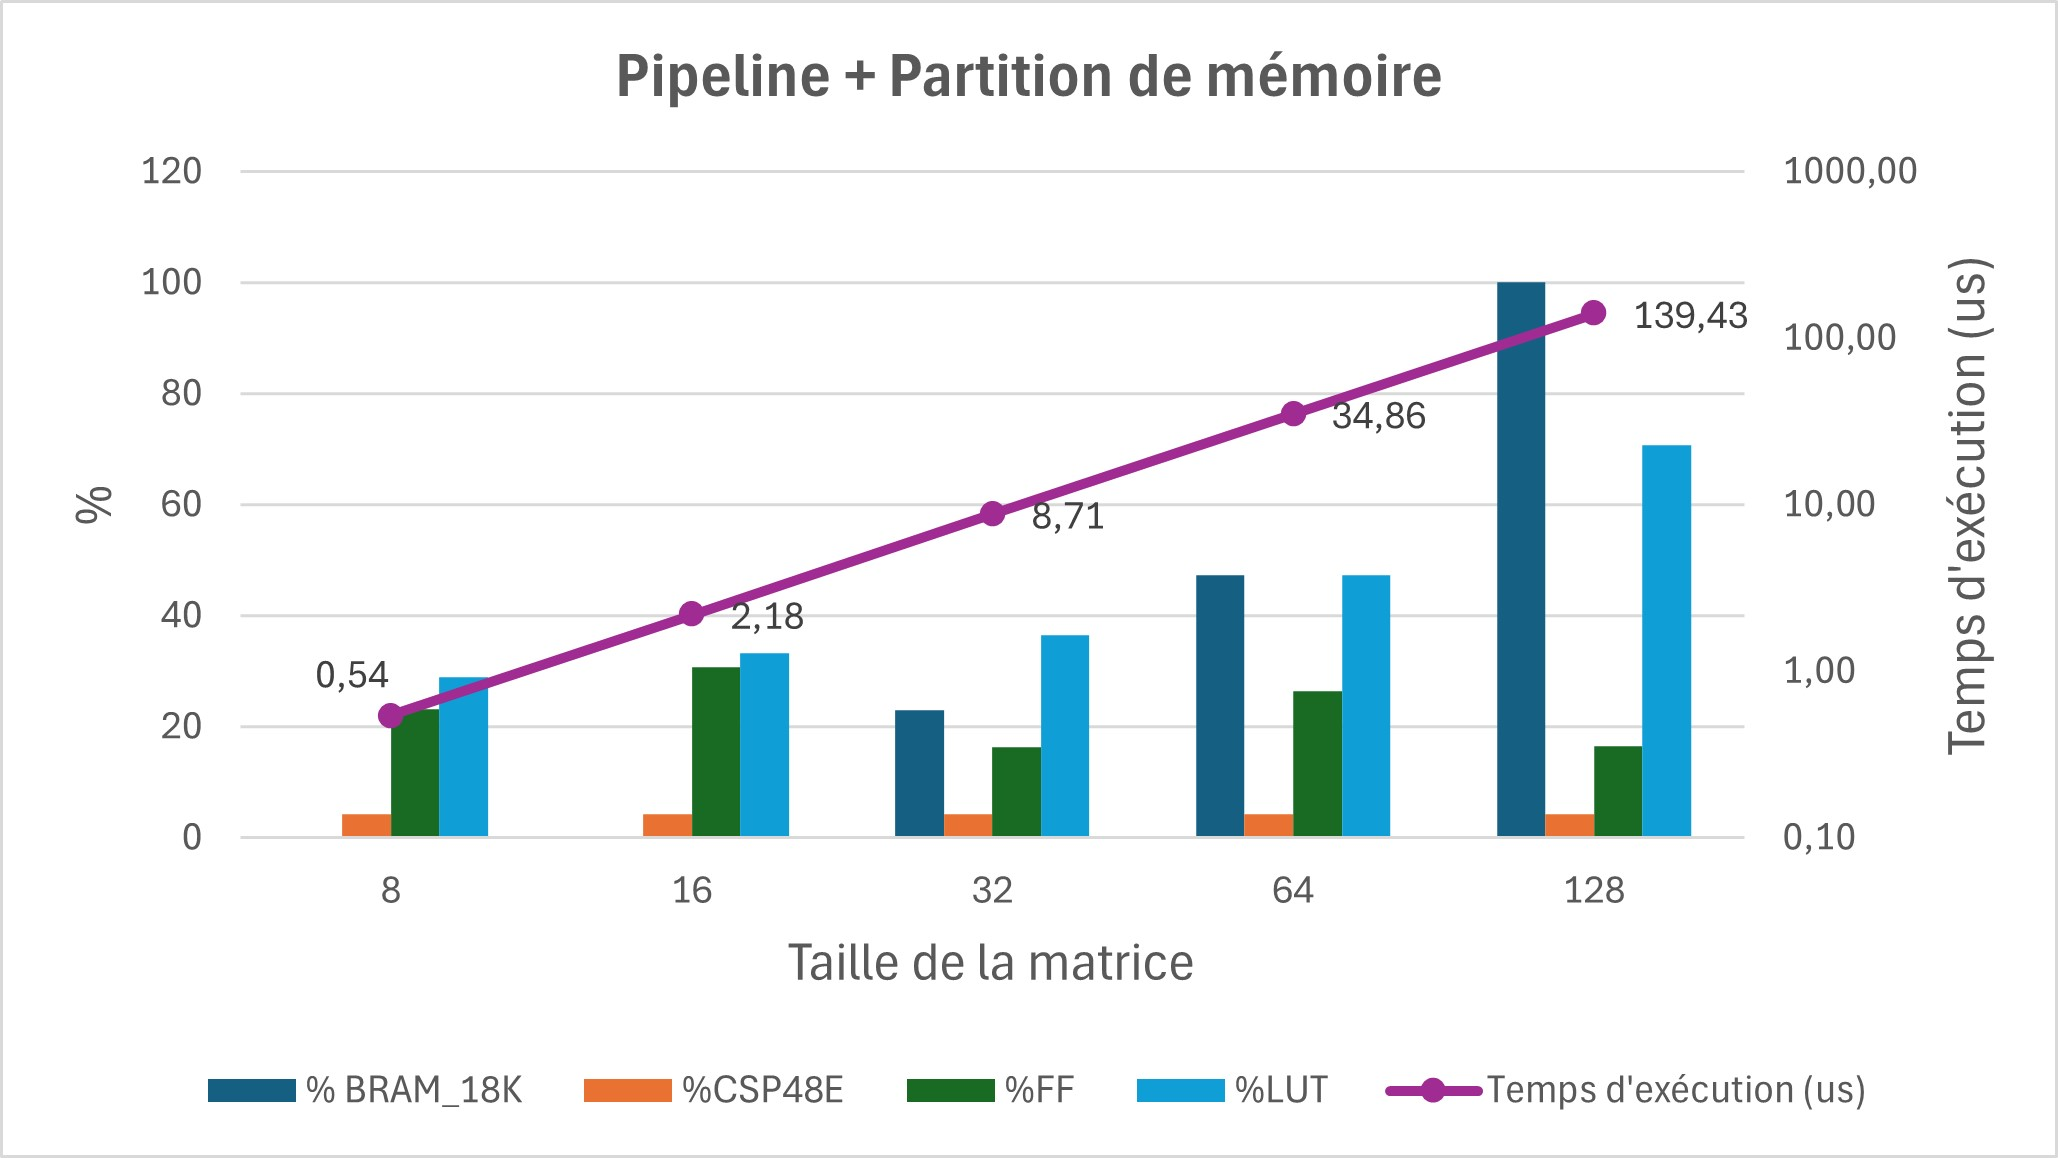
\includegraphics[width=1\columnwidth]{Images/Bloques_R_2.jpg}
    \caption{Blocs Réordonné avec partitionnement de pipelines et de tableaux.}
    \label{fig:15}
\end{figure}

Semblable à la version non réordonnée, la consommation de ressources est plus élevée dans cette optimisation sans qu’une amélioration substantielle des temps d’exécution ne soit observée. Encore, les routines de partition de mémoire augmentent l'utilisation des ressources par rapport à l'optimisation de pipeline simple.

\begin{figure}[H]
    \centering
    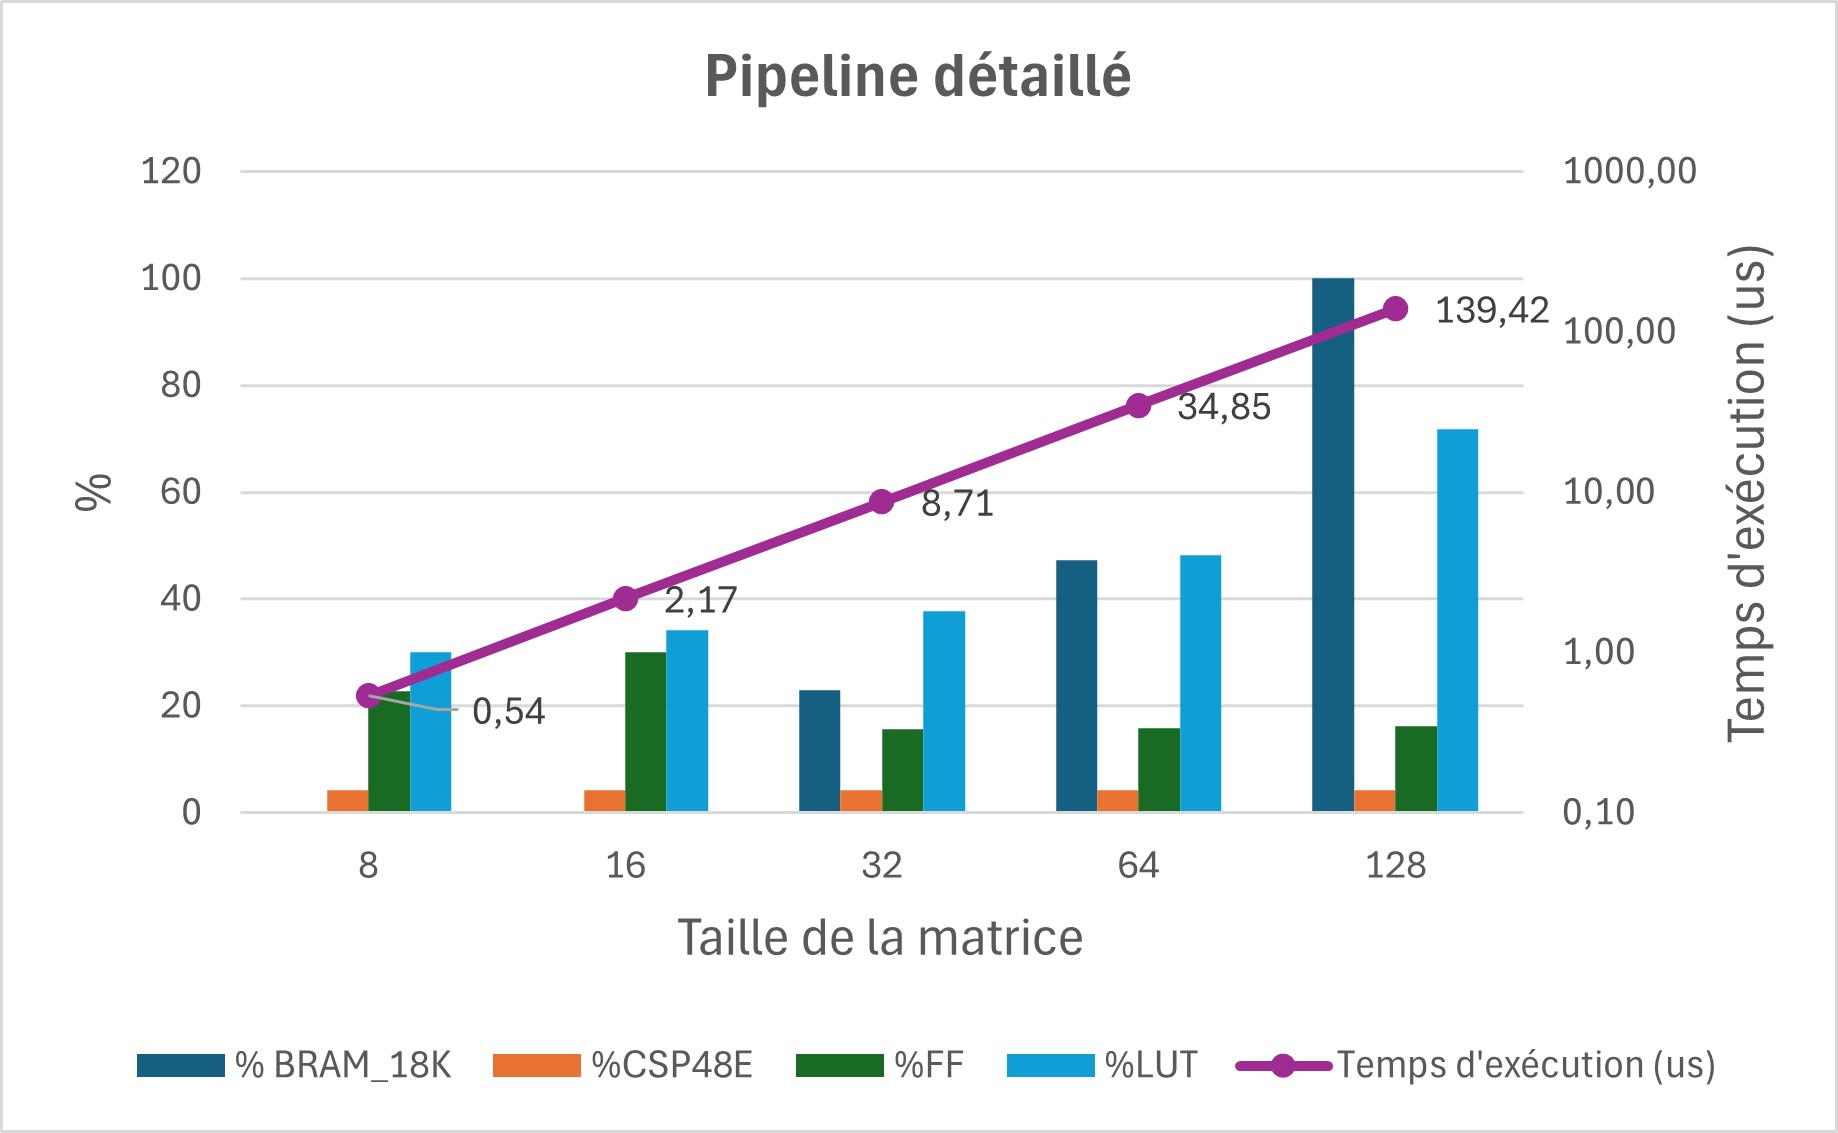
\includegraphics[width=1\columnwidth]{Images/Bloques_R_3.jpg}
    \caption{Blocs Réordonné avec pipeline détaillé.}
    \label{fig:16}
\end{figure}

Bien que les ressources matérielles augmentent par rapport à la version bloc standard, les temps d'exécution sont pratiquement les mêmes.

En général, les optimisations liées à une pipeline représentent un gain significatif de temps, bien comme consomment plus de ressources. 

\end{document}
